\documentclass[12pt,oneside,bibtotoc,liststotoc]{scrbook}
% \usepackage[utf8]{inputenc}
\usepackage{lmodern}
\usepackage[T1]{fontenc}
\usepackage[usenames,dvipsnames]{xcolor}
\usepackage{graphicx}
\usepackage[english]{babel}
\usepackage{a4wide}
\usepackage{parskip}
\usepackage[bookmarks]{hyperref}
\usepackage{fancyhdr}
\usepackage[right]{eurosym}
\usepackage{amsmath}
\usepackage{amssymb}
\usepackage[toc,page]{appendix}
\usepackage{todonotes}
\usepackage{acronym}
\usepackage{subfiles}


\usepackage[numbers]{natbib}
% \DeclareUnicodeCharacter{2192}{ to}

\usepackage{listings}

\usepackage{lstautogobble}
\usepackage[edges]{forest}
\usepackage{array}
\usepackage{longtable}
\usepackage{listings}
\usepackage{color}

\colorlet{punct}{red!60!black}
\definecolor{background}{HTML}{EEEEEE}
\definecolor{delim}{RGB}{20,105,176}
\colorlet{numb}{magenta!60!black}
\lstdefinelanguage{json}{
    basicstyle=\footnotesize\ttfamily,
    numbers=left,
    tabsize=2,
    lineskip={-1.0pt},
    numberstyle=\scriptsize,
    stepnumber=1,
    numbersep=8pt,
    showstringspaces=false,
    breaklines=true,
    frame=lines,
    backgroundcolor=\color{background},
    literate=
      *{:}{{{\color{punct}{:}}}}{1}
      {,}{{{\color{punct}{,}}}}{1}
      {\{}{{{\color{delim}{\{}}}}{1}
      {\}}{{{\color{delim}{\}}}}}{1}
      {[}{{{\color{delim}{[}}}}{1}
      {]}{{{\color{delim}{]}}}}{1},
}
\lstdefinelanguage{rdf}{
    basicstyle={\footnotesize\ttfamily},
    lineskip={-1.0pt},
    numbers=left,
    numberstyle=\scriptsize,
    stepnumber=1,
    numbersep=8pt,
    showstringspaces=false,
    breaklines=true,
    frame=lines,
    tabsize=2,
    backgroundcolor=\color{background},
    keywordstyle={\bfseries\color{Blue}},
    commentstyle={\color{Red}\textit},
    stringstyle=\color{Magenta},
    morekeywords={ql,rml,rr,schema},
    moredelim=*[s][\ttfamily]{:}{:} %Newly added line
}
\lstdefinelanguage{xml}{
    basicstyle={\footnotesize\ttfamily},
    lineskip={-1.0pt},
    numbers=left,
    tabsize=2,
    numberstyle=\scriptsize,
    stepnumber=1,
    numbersep=8pt,
    showstringspaces=false,
    breaklines=true,
    frame=lines,
    backgroundcolor=\color{background},
    keywordstyle={\bfseries\color{Blue}},
    commentstyle={\color{Red}\textit},
    stringstyle=\color{Magenta},
    morekeywords={ServiceProvider,Document,Address,Service,Product,Occupancy,Price},
    moredelim=*[s][\ttfamily]{:}{:} %Newly added line
}
\newcommand\tab[1][1cm]{\hspace*{#1}}
\lstset{
	basicstyle=\ttfamily\small,
	showspaces=false,
	numbers=left,
	breaklines = true,
	showstringspaces=false
}

\pagestyle{headings}
\setlength{\textwidth}{15cm}
\setlength{\textheight}{22.5cm}
\setlength{\oddsidemargin}{1cm}
\setlength{\evensidemargin}{0cm}
\begin{document}


\thispagestyle{empty}
\begin{center}
\LARGE{Leopold-Franzens Universität Innsbruck\\
Faculty for Mathematics, Computer Science and Physics}\\[3ex]
\large{Institut for Physics}\\[2ex]
\large{Theoretical Plasma Physics}
\end{center}
\medskip

\begin{center}

\includegraphics[width=3cm]{Logo}
\vspace{1.5cm}

\textbf{\LARGE{Masterthesis}}
\medskip\par
\textbf{\normalsize{zur Erreichung des akademischen Grades}} \\[3ex]
\textbf{\Large{Master of Science}}
\vspace{2cm}

\textbf{\Large{Title of the work}}
\bigskip\par
von \par
\large{Jascha Riedel}\\
(Matr.-Nr.: 0123456789)
\end{center}
\vspace{1cm}

\begin{tabular}{ll}
  Submission Date:  & \today \\
  Supervisor: & Alexander Kendel \\
\end{tabular}

\newpage

\vspace*{5cm}

\begin{center}
\LARGE{Eidesstattliche Erklärung}\\
\end{center}
\vspace{1cm}


\begin{quote}
\emph{Ich erkläre hiermit an Eides statt durch meine eigenhändige Unterschrift, dass ich die vorliegende Arbeit selbstständig verfasst und keine anderen als die angegebenen Quellen und Hilfsmittel verwendet habe. Alle Stellen, die wörtlich oder inhaltlich den angegebenen Quellen entnommen wurden, sind als solche kenntlich gemacht.
\\Ich erkläre mich mit der Archivierung der vorliegenden Bachelorarbeit einverstanden.
}
\end{quote}
\vspace{2.5cm}

\begin{flushleft}
\begin{tabular}{lll}
Ort und Datum: & & \rule{7cm}{0.4pt}\\[7ex]
Unterschrift: & & \rule{7cm}{0.4pt}
\end{tabular}
\end{flushleft}

\thispagestyle{empty}

\renewcommand{\baselinestretch}{1.00}\normalsize

\tableofcontents
\setcounter{page}{1}
\pagenumbering{Roman}
\listoffigures
\renewcommand{\baselinestretch}{1.5}\normalsize

\newpage
\setcounter{page}{1}
\pagenumbering{arabic}

\chapter*{Zusammenfassung}
\addcontentsline{toc}{chapter}{Zusammenfassung}
Deutsches Abstract

\begin{otherlanguage*}{english}
\chapter*{Abstract}
\addcontentsline{toc}{chapter}{Abstract}
Englisches Abstract
\end{otherlanguage*}





\chapter{Introduction}

\chapter{Theory Physics}

\section{Full-F Gyrofluid Equations}
The following section describes a reduced set of equations derived from the Full-F Gyrofluid Equations published by J. Madsen \cite{doi:10.1063/1.4813241}.
\todo[]{Find out where}The simulation is currently limited to the Isothermal Full-F Gyrofluid Equations as they have been derived in

\section{Coordinate System}
\subfile{coordinateSystem}
% \documentclass[master.tex]{subfiles}
 
\begin{document}


A Flux-Tube coordinate system is employed.
The coordinate system in the simulation code has the letters $z$ $x$ and $y$. They map to the following coordinates as they are introduced in \cite{doi:10.1063/1.1335832}.
\begin{itemize}
    \item $x = r - a$   (i. e. radial distance)
    \item $y = q\theta - \xi$ (i. e. shear shifted (by $q\theta$) poloidal angle)
    \item $z = \theta$ (i. e. torodial angle/flux surfaces)
\end{itemize} 
where $a:=minor\, Radius$, $\xi \in [0,2\pi]$, $\theta \in [-\pi,\pi]$ and $\theta = 0$ is the magnetic surface at the \textit{outboard-midplane}.\\
Thus if we chose $z=[0,8]$ we have eight $x-y$ simulation planes evenly distributed around the torus following the magnetic field lines (i. e. field-aligned).The deformation of the $x-y$ planes is accounted for by the shift-parameter which influences the parallel derivatives \cite{ScootShiftedMetric}.\newline
It is noteworthy that the $y$ coordinate doesn't actually cover the full poloidal disc. This might seem counter intuitive but as is show in \cite{ScottFluxTube} a carefully set of modes may be \textit{picked} out that covers the turbulence we are interested in. In the reference this is done by the analysis of the fourier decomposition of a general \textit{physical quantity} that obeys continuity constraints in the geometry (for instance the electron density $n_e$).
This constraint on the allowed wavelengths (modes) justifies the use of a Flux-Tube coordinate system where the \textit{Tube} follows a magnetic field line around the torus and does not cover the entire flux surface. Therefore the simulation doesn't cover a complete torus but only models a smaller region that covers large scale $k_\parallel$ modes (parallel to the magnetic field) and small scale $k_\perp$ modes (perpendicular to the magnetic field). Using this reduced simulation area prevents the possible introduction of non physical modes in parallel direction.


\end{document}
\section{Isothermal 3D Full-F Gyrofluid Equations}
\label{sec:isothermalequations}
\subfile{isothermal-full-f-gyrofluid-equations}
% \documentclass[master.tex]{subfiles}
 
\begin{document}

The equations are stated without proper derivation (a mathematical derivation can be found in \cite{HeldDisseration}). It is essentially a set of six equations. Two density equations (\autoref{eq:electron_density}, \autoref{eq:ion_density}), two parallel velocity equations (\autoref{eq:electron_velocity}, \autoref{eq:ion_velocity}), the polarization equation (\autoref{eq:polarization}) and a closure approximation for the gyro averaging operator $\Gamma_1$.

\subsection{Density Equations}

\begin{align}
    \overbrace{\partial_t n_e}^{Variation} &=
    \overbrace{-\delta^{-1} \left[\Tilde{n}_e, \phi \right]_{\perp}}^{\perp \, Convection}
    \overbrace{
    - \mathcal{K}(\Tilde{n}_e)
    - \mathcal{K}(\phi)
    }^{\perp \, Curvature}
    \overbrace{
    - \frac{1}{B(z)}\nabla_\parallel (v_{e\parallel} n_e)
    }^{\parallel \, Current\,\, Divergence}
    \overbrace{
    + \nu_\parallel \nabla_\parallel^2\Tilde{n}_e
    - \nu_\perp \Delta^2_\perp\Tilde{n}_e
    }^{Artificial\,\, Viscosities}
    \label{eq:electron_density}
    \\
    \partial_t N_i &=
    -\delta^{-1} \left[\Tilde{N}_i, \psi \right]_{\perp}
    - \mathcal{K}(\Tilde{N}_i)
    - \mathcal{K}(\Tilde{\psi_i})
    - \frac{1}{B(z)}\nabla_\parallel (v_{i\parallel} N_i)
    + \nu_\parallel \nabla_\parallel^2\Tilde{N}_i
    - \nu_\perp \Delta^2_\perp\Tilde{N}_i \label{eq:ion_density}
\end{align}

where

\begin{align}
    \mathcal{K}(\lambda) &= (\kappa_x \partial_x + \kappa_y \partial_y)\,\lambda\\
    \kappa_x &= mcv \cdot sin(\theta)\\
    \kappa_y &= mcv \cdot cos(\theta) + shear\\
    \left[A, B\right]_\perp &= \partial_x A \cdot \partial_y B - \partial_x B \cdot \partial_y A\\
    \nabla_\parallel \lambda &= \Tilde{\partial_{z}} \lambda
\end{align}
\begin{itemize}
    \item $\Tilde{\partial_{z}}$ represents the shear-shifted derivative in z-direction.
    \item $\Tilde{X} := ln(X)$
    \item $B(z) := $ Magnetic-Field in z-plane
\end{itemize}


\autoref{eq:electron_density} represents the evolution of the electron density field.
\autoref{eq:ion_density} represents the evolution of the gyrocenter density of gyro-averaged species (i. e. ions). Since the electrons gyro-radius is small compared to the ion gyro-radius, the effects of electron gyration can be neglected.\todo{Find a reference or write equations down} \newline
The last two terms in both equations are needed for numerical stability of our schemes but may be regarded as sinks.


\subsection{Parallel Velocity Equations}
For the velocities only the parallel part needs to be solved explicitly. The perpendicular part is purely $\mathrm{E}\times \mathrm{B}$ convection which is contained in the electric potential $\phi$. This is a result of the \textit{drift approximation} where the strong magnetic field in parallel direction forces the particles to a fast gyration around the field lines. The perpendicular velocity can then be calculated from the electric and magnetic field considering the Lorentz Force and is decoupled from the parallel velocity.


\begin{align}
\begin{split}
    \alpha_e &=  -\frac{\mu_e \hat{\epsilon}}{\delta} \left[v_{e\parallel}, \phi_\perp\right]_\perp
    - 2 \cdot \tau_e \mu_e \hat{\epsilon} \cdot \mathcal{K}( v_{e\parallel})
    - 2 \cdot \tau_e^2 \mu_e \hat{\epsilon} \cdot \mathcal{K}(\Tilde{n}_e)
    - 0.5 \cdot \tau_e \mu_e \hat{\epsilon} \cdot \mathcal{K}( \phi)\\
    & \quad - \nabla_\parallel (\phi + \tau_e n_e)
    - \hat{c} \cdot \mathrm{J}
    + \nu_\parallel \nabla_\parallel^2\Tilde{\alpha}_e 
    - \nu_\perp \Delta^2\Tilde{\alpha}_e \label{eq:electron_velocity}
\end{split}\\
\begin{split}
    \alpha_i &= -\frac{\mu_i \hat{\epsilon}}{\delta}  \left[v_{i\parallel}, \phi_\perp\right]_\perp
    - 2 \cdot \tau_i \mu_i \hat{\epsilon} \cdot \mathcal{K}(v_{i\parallel})
    - 2 \cdot \tau_i^2 \mu_i \hat{\epsilon} \cdot \mathcal{K}(N_i)
    - 0.5 \cdot \tau_i \mu_i \hat{\epsilon} \cdot \mathcal{K}(\psi)\\
    &\quad - \nabla_\parallel (\psi + \tau_i N_i)
    - \hat{c} \cdot  \mathrm{J}
    + \nu_\parallel\nabla_\parallel^2\Tilde{\alpha}_i 
    - \nu_\perp \Delta^2\Tilde{\alpha}_i \label{eq:ion_velocity}
\end{split}
\end{align}

where ($s$ denotes electron and ion species)

\begin{itemize}
    \item $\alpha_s := \mu_s \hat{\epsilon} \cdot v_{s\parallel} + \hat{\beta} \cdot A_{\parallel}$
    \item $\mathrm{J} := \sum_s z_s \cdot n_s \cdot v_{s\parallel}$
    \item $z_s :=$ charge of species particles (i. e. -1 for electrons)
\end{itemize}

As a simplification we assume $\hat{\beta} \approx 0$ and thus Amperes Law is not stated here. Nonetheless to closely represent the equations implemented in the simulation code the $\alpha$-notation is used here.

\subsection{Polarization Equation}

\begin{align}
    \nabla \cdot \left( \sum_s \mu_s n_s \right) \nabla \phi &= z_e n_e + \sum_i z_i \, \cdot \, N_i \label{eq:polarization}
\end{align}
The polarization equation connects the individual species by the quasi-neutrality condition for a plasma. This is a non linear partial differential equation of second order. To handle the non linearity a typical assumption is that $\sigma := \sum_s \mu_s n_s$ can be expanded in space and or time ($\sigma \approx \sigma_0 + \sigma_1 \epsilon + ...$ where $\epsilon$ represents the Larmor radius length scale) and that $\sigma_1 \epsilon \ll \sigma_0$ as well as $\sigma_0$ is constant. Three different simplifications of that kind will be presented in \autoref{sec:polarization-linearizations} and evaluated in \autoref{sec:polarization_equation_evaluation}. 


\begin{blockquote}
    On the right hand side essentially stands the (gyro-averaged) charge distribution. The left-hand side contains \ac{FLR} effects via the non-linearity.
\end{blockquote}

\subsection{Gyro-Averaging Operator}
Since we have a Gyrofluid model we need a transformation from the actual quantities into the gyro averaged quantities. In our case we only need $\Gamma_1$ and $\Gamma_1^\dagger$. A derivation and further explanation can be found in \cite{HeldDisseration}.
\begin{align}
    \label{eq:gyro-averaging-opeartor}
    \Gamma_1 = \left(1- \frac{1}{2} \rho^2 \nabla_\perp^2\right)^{-1}
\end{align}


\section{Approximations of the Polarization Equation} \label{sec:polarization-linearizations}
\autoref{eq:polarization} is a general form of the more familiar Poisson equation
\begin{equation}\label{eq:linear-poisson-equation}
    \Delta \Psi = \rho 
\end{equation}
whereas \autoref{eq:polarization} has the following form
\begin{equation}\label{eq:general-poisson}
    \nabla N(x,y) \nabla \Psi = \rho(x,y).
\end{equation}

Solving \autoref{eq:linear-poisson-equation} is much simpler and thus it is desirable to bring \autoref{eq:general-poisson} into the same form. Presented are three different linearizations. These are evaluated and compared later.

\subsection{Constant Background Linearization \textit{(Local Model)}}

In \autoref{eq:general-poisson} we assume $N(x,y, t) \approx \overline{N}_0$ for all times where $\overline{N}_0=\frac{1}{L_yL_x}\int_{[x,y]} N(x,y, t = 0) dx dy$. \autoref{eq:general-poisson} reduces to:
\begin{equation}
    \Delta \Psi(x,y,t) = \frac{\rho(x,y,t)}{\overline{N}_0}
\end{equation}
This approximation would be valid if $N(x,y, 0) \approx N(x,y,t)$ and $\nabla N(x,y,0) \approx 0$. In some contexts this is also referred to as  $\delta-f$ or \textit{local model} whereas the non linearized form is called a \textit{global model}.

\subsection{Time-independent Radial Background Profile}
In \autoref{eq:general-poisson} we assume $N(x,y,t) \approx \left<N(x,t = 0)\right>_y$. This reduces the general poisson equation to:
\begin{equation}
    \partial_x \left<N(x,t = 0)\right>_y \partial_x \Psi(x,y,t) + \left<N(x,t = 0)\right>_y \partial_{yy} \Psi(x,y,t) = F(x,y,t);
\end{equation}
This would be valid if $\partial_y N \approx 0$ and $N(x,y,t) \approx N(x,y, t= 0)$.

\subsection{Time-dependent Radial Background Profile}
In \autoref{eq:general-poisson} we assume $N(x,y,t) \approx \left<N(x,t)\right>_y$. This reduces the general poisson equation to:
\begin{equation}
    \partial_x \left<N(x,t)\right>_y \partial_x \Psi(x,y,t) + \left<N(x,t)\right>_y \partial_{yy} \Psi(x,y,t) = F(x,y,t);
\end{equation}
This would be valid if $\partial_y N \approx 0$.
\newline
Evaluation and results are found in \autoref{sec:polarization_equation_evaluation}. It should be noted that the first and second linearization naturally depend on the initial density profile and thus it needs to be chosen carefully.

\end{document}


\section{Fluid Dynamics}
\label{sec:fluid-dynamics}
\subfile{fluid-dynamics}
% \documentclass[master.tex]{subfiles}
 
\newcommand{\meanxy}[1]{\left<#1\right>_{z,y}}
\begin{document}


\subsection{Connection to Navier-Stokes}
\label{sec:connection_navier_stokes}

The structure of the density and velocity equations closely resembles that of the incompressible Navier-Stokes equations.
There are some transformations necessary to see the connection and we restrict ourselves to the 2D case. We start with the incompressible Navier Stokes equations.

\begin{align}
    \partial_t v &= - \nabla p - v \cdot \nabla v + \Delta v
\end{align}

In the two-dimensional case this transformation
\begin{align}
    v_x &= \partial_y \psi \\
    v_y &= -\partial_x \psi \\
    \xi &= \Delta \psi
\end{align}
yields the following pressure-free formulation of the Navier-Stokes equations.

\begin{align}
    \partial_t \xi &= \left( \partial_x \psi \partial_y \xi - \partial_y \psi \partial_x \xi  \right) + \Delta \xi\\
    \partial_t \xi &= - \left[\xi, \psi\right] + \Delta \xi \label{eq:vorticity-streamline-potential} \\
\end{align}

In a $\delta$f framework and without thermal effects ($\tau_i = 0$) the evolution equations for the (gyro-averaged) densities (\autoref{eq:electron_density} and \autoref{eq:ion_density}) can be combined (considering the charge of the species $z_s$) and transformed into  \autoref{eq:vorticity-streamline-potential} by using a $\delta$f form of the polarization equation (\autoref{eq:polarization}).\newline
This only serves as motivation to use terminology from flow equations. We can now define turbulent and zonal flow in the following way:

\begin{align}
    \Gamma(z,x,y) &= \partial_y \phi_e :\, Turbulent\,Flow\\
    \Lambda(z,x,y) &= \partial_x \phi_e :\, Poloidal\,Flow
\end{align}

Here the turbulent flow gives us information on how much of our quantities is transported outwards into the \ac{SOL} by $\mathrm{E}\times\mathrm{B}$ convection and the poloidal flow represents perpendicular (to the magnetic field) transport parallel to the separatrix.

\subsection{Simulation Quantities}\label{sec:simulation_quantities}



In order to characterize the simulation results some quantities are defined. Often we are interested in the radial profile of our quantities thus we define the radial profile of a quantity $\mathcal{A}$, as:
\begin{equation}
    \left<\mathcal{A}\right>_y = \frac{1}{L_y} \int_{[y]} A(z,x,y) \, dy
\end{equation}
which essentially is the mean value over the y-direction,
and the zonal profile as:
\begin{equation}
    \left<\mathcal{A}\right>_{z, y} =\frac{1}{L_yL_z} \int_{[z, y]} A(z,x,y) \, dzdy
\end{equation}
Here $[z,x,y]$ should represent the full domain and $[z,y]$ the subdomain $[L_z \times L_y]$. Further on $S$ is defined as the separatrix position in $x$-direction to define two subsets of the full domain by $[z,y,x\leq S]$ as the core region and $[z,y,x > \mathcal{S}]$ as the \ac{SOL} region.



We now define these quantities for further evaluation in \autoref{sec:polarization_equation_evaluation}:

\begin{itemize}
    \item $\overline{\Gamma}_{Core} \propto  \left<\Gamma\right>_{z,y, x \leq \mathcal{S}}$ : \textit{Turbulent Flow in Core Plasma}
    \item  $\overline{\Gamma}_{SOL} \propto  \left<\Gamma\right>_{z,y, x > \mathcal{S}}$ : \textit{Turbulent Flow in \ac{SOL} Plasma}
    \item $\Gamma^*(x) \propto \left<\Tilde{n}_s \cdot \Gamma\right>_{z,y}$ : \textit{Turbulent Flux at $x$}
    \item $\meanxy{\phi_e}$ : \textit{Zonal Potential}
    \item $\partial_x \meanxy{\phi_e}$ : \textit{Zonal Flow}
    \item $\partial_{xx}\meanxy{\phi_e}$ : \textit{Zonal Vorticity}
    \item $E_n \propto \left<\sum_s  \tau_s n_s^2 \right>_{z, x, y,}$ : \textit{Full Density weighted by temperature ratio}
    \item $\mathrm{E}_{v_\parallel} = \hat{\epsilon} \cdot \left<\sum_s \mu_s v_{s\parallel} \right>_{z, x, y}$ : \textit{Parallel Kinetic Energy}
\end{itemize}


\end{document}



\chapter{Theory Numerics}
\section{Discretization}
\subfile{discretization}
% \documentclass[master.tex]{subfiles}
 
\begin{document}


The simulation domain is mapped to an equidistant rectangular grid in x-y direction. The distance between each grid point is fixed by a single parameter forcing both to be equal ($h_x = h_y$). This reduces the complexity of some finite differences schemes. In z-direction the distance between each grid point simply equals the discretization of a unit circle ($h_z= \frac{2\pi}{n_z}$ or going around a torus once poloidally).

\end{document}
\section{Boundary Values}
\subfile{BoundaryValues}
% \documentclass[master.tex]{subfiles}
 
\begin{document}

To treat the domain boundaries numerically ghost cells are implemented. Currently the the simulation needs two ghost cells in every direction.

\subsection{X-Direction}
For the densities the following boundary conditions are employed:
\begin{equation}
    n_s(x) = \begin{cases}
        2 \cdot n_{s0}(0) - n_{s0}(-x) &\colon for \, x < 0 \\
        2 \cdot n_{s0}(x_L) - n_{s0}(2x_L-x) &\colon for \, x > x_L \\
    \end{cases}
\end{equation}
This enforces a mixed Dirichlet-Neumann boundary condition.
The parallel velocities are forced to equal zero at the boundaries.
For the potential a special boundary condition is employed:
\begin{align}
    \phi_e(x) = 0 \qquad &\colon for \, x = 0\\
    \partial_x\phi_e(x) = 0 \qquad &\colon for \, x = x_L \label{eq:boundary-potential-right}
\end{align}
The first condition fixes the absolute value of the potential and is necessary for the numerical solver to converge. This can be seen as a Coulomb gauge. This fixing may artificially create high gradients at the $x=0$ boundary and thus one needs to extend the boundary conditions of the densities into to the domain. The second condition forces zero gradients in x-direction on the $x=x_L$ boundary. Since only the gradient of the potential appears as driving term in the equations those conditions for the potential move artificial dynamics to the left core region where they are easier to handle. 

\subsection{Y-Direction}
In Y-Direction (which is perpendicular to X but not in toroidal direction) closed boundary conditions are implemented. One of the consequences is that there is an \textit{in and out flow} of vortices simulating turbulence incoming from the not simulated area of the poloidal slice. The length of Y-Direction needs to be chosen carefully such that vortices that are mirrored to the opposite do not interfere with themselves and that all important modes are possible (4x times x size) \cite{ScottFluxTube} \cite{ScottComputationMagneticallyConfinedPlasmas}.
\subsection{Z-Direction}
In Z-Direction there is a differentiation whether the X-coordinate lies in/on or outside the separatrix (last closed magnetic field line/flux surface).
\paragraph{In/On Separatrix}
Here we assume closed field lines and thus employ closed boundary conditions.
\paragraph{Outside of Separatrix}
To simulate \todo{Ref-Ribero-Scott} divertors outside the separatrix so called \textit{limiters} are simulated by not connecting the $z=0 \And z=n_z$ planes but rather using open boundary conditions for the densities and potential, and Dirichlet boundary conditions for the velocities. The situation is illustrated in \autoref{fig:boundary_conditions_z}
\begin{figure}[ht]
    \centering
    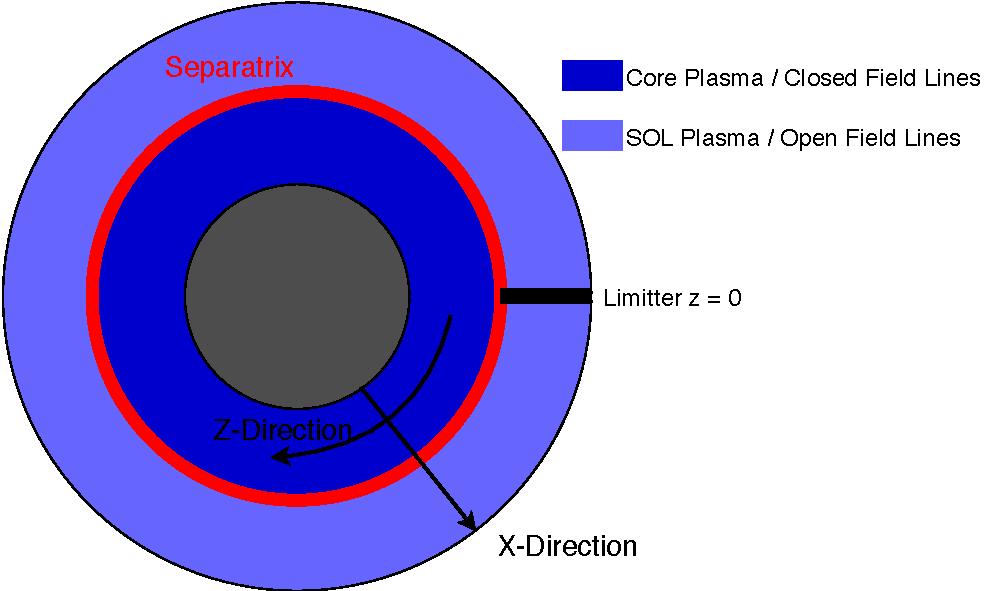
\includegraphics[width=\linewidth]{pdfs/boundary_conditions_z.pdf}
    \caption{Visualization of tokamak with separatrix and limiter}
    \label{fig:boundary_conditions_z}
\end{figure}

\end{document}
\section{Numerical Methods}
\subfile{numericalMethods}
% \documentclass[master.tex]{subfiles}
 
\begin{document}

There are three different main problems to solve in this simulation.
\begin{itemize}
    \item Derivatives (parallel and perpendicular)
    \item Time Integration
    \item Poisson/Laplace equation solving
\end{itemize}

\subsection{Derivatives}
Since a simple grid is chosen for discretization standard finite-differences schemes are used for the derivatives and a special scheme for the poisson brackets (arakawa-scheme) \cite{arakawa}.\newline
These are the discretizations used throughout the simulation:\newline
\textit{Coordinates not involved are omitted for readability. $T_{i + 1} = T_i + h_T$ for T in $\{z, x, y\}$}
\begin{itemize}
    \item Perpendicular Gradient $\nabla_{\perp} = \vec{n}\cdot\nabla$\\
     \begin{small}
        \begin{equation}
        \begin{split}
            \nabla_{\perp} f(z, x_i,y_j) &\approx  \quad\frac{-f(x_{i+2},y) + 8 \cdot f(x_{i + 1}, y) -  8 \cdot f(x_{i - 1}, y) + f(x_{i - 2}, y)}{6 \cdot h_x} \\
            &\quad + \frac{-f(x,y_{i + 2}) + 8 \cdot f(x, y_{i + 1}) -  8 \cdot f(x, y_{i - 1}) + f(x, y_{i - 2})}{6 \cdot h_y}\\
            &\quad + O(h_x^4) + O(h_y^4)
        \end{split}
        \end{equation}
    \end{small}
    \item Parallel Gradient $\nabla_{\parallel} = \vec{e_z}\cdot\nabla = \partial_z$\\
    \begin{equation}
        \nabla_{\parallel} f(z_i,x,y) \approx \frac{-f(z_{i+2}) + 8 \cdot f(z_{+1}) - 8 \cdot f(z_{-1}) + f(z_{-2})}{12 \cdot h_z} + O(h_z^4)
    \end{equation}
    \item Second parallel derivative $\partial_z^2$\\
    \begin{equation}
           \partial_z^2f(z_i,x,y) \approx \frac{f(z_{i+1})-2\cdot f(z_i)+ f(z_{i-1})}{h_z^2} + O(h_z)
    \end{equation}
    \item Fourth derivative in perpendicular direction $\nabla_\perp \cdot \nabla_\perp$\\
    \begin{footnotesize}
    \begin{equation}
    \begin{split}
    \nabla_\perp^2f(z,x_i,y_j) \approx \frac{f(x_{i+2},y_j) - 4 \cdot f(x_{i+1},y_j) +6\cdot f(x_i,y_j) -4 \cdot f(x_{i-1},y_j) + f(x_{i-2}, y_j)}{h_x^4}  \\ + \frac{f(x_{i+2},y_j) - 4 \cdot f(x_{i+1},y_j) +6\cdot f(x_i,y_j) -4 \cdot f(x_{i-1},y_j) + f(x_{i-2}, y_j)}{h_x^4}  \\  + O(h_x^2) + O(h_x^2)
    \end{split}
    \end{equation}
\end{footnotesize}      %$[f(x,y),g(x,y)]_\perp = \partial_x f \partial_y g - \partial_y f \partial_x g$
    \item Poisson Bracket \\
    \begin{footnotesize}
        \begin{equation}
            \begin{split}
                [f(x,y), g(x,y)]_\perp = -\frac{1}{12h_xh_y} & [
                    (g_{i, j-1} + g_{i+1,j-1} - g_{i, j+ 1} - g_{i+1,j+1})(f_{i+1,j}-f_{i, j}) \\
                    &+ (g_{i-1,j-1}+g_{i,j-1}-g_{i-1,j+1} - g_{i,j+1})(f_{i,j}-f_{i-1,j})\\
                    &+ (g_{i+1,j}+g_{i+1,j+1}-g_{i-1,j}-g_{i-1,j+1})(f_{i,i+1}-f_{i,j})\\
                    &+ (g_{i+1,j+1}+g_{i+1,j}-g_{i-1,j-1}-g_{i-1,j})(f_{i,j}-f_{i,j-1})\\
                    &+ (g_{i+1, j} - g_{i, j + 1})(f_{i+1,j+1}-f_{i,j})\\
                    &+ (g_{i, j-1} - g_{i-1, j})(f_{i,j}-f_{i-1,j-1})\\
                    &+ (g_{i,j+1}-g_{i-1,j})(f_{i-1,j+1}-f_{i,j})\\
                    &+ (g_{i+1, j} - g_{i,j-1})(f_{i,j}-f_{i+1,j-1}) ]
            \end{split}
        \end{equation}
    \end{footnotesize}


\end{itemize}

\subsection{Time Integration - Karniadakis Scheme}
The time stepping is implemented using a Karniadakis scheme of 3rd order \cite{KARNIADAKIS1991414}.
It is applied to the density and velocity equations described in \autoref{sec:isothermalequations}.
In our case it iterates an equation of form
\begin{equation}
    \partial_t \Phi = F(\Phi) - \lambda_s
\end{equation}
where $\lambda_s$ represents sources and sinks and $n$ denotes the time step in the following way :
\begin{equation}\label{eq:karnidakis-scheme}
\begin{split}
    \Phi^{n + 1} = \quad &\frac{18}{11} \Phi^{n} - \frac{9}{11} \Phi^{n-1} + \frac{2}{11}  \Phi^{n-2}\\
     + &\frac{6}{11}\Delta t \cdot (3 \cdot F(\Phi)^{n+1} - 3 \cdot F(\Phi)^{n} + F(\Phi)^{n-1} + \lambda_s)
\end{split}
\end{equation}
This scheme has been shown to be stable at high \ac{CFL} number for the incompressible navier-stokes equation \cite{KARNIADAKIS1991414}.

\subsection{Poisson Equation solver}
There are two poisson-like equations to solve. The frist one is necessary to apply the padé-approximation of the gyro-averaging operator and is solved using a fourier decomposition. The second one is the polarization equation as described in \autoref{sec:isothermalequations} and is solved using a \ac{SOR} gauss-seidel-iterator.

\subsubsection{Gyro-Averaging - Fourier Solver}
The gyro-averaging operation has the form:
\begin{equation}
    \alpha \Delta U(x, y) = F(x, y)
\end{equation}
This equation is solved using Fourier-Method as it is described here \cite{fft-poisson}. To achieve a periodic function in x-direction the domain is extended in this direction before computation. The transformation rule is:
\begin{equation}
\label{eq:gyro-transformation}
\begin{split}
    t\colon [n_x, n_y] & \to [4 \cdot n_x, n_y]\\
    f(x, y) &\mapsto \begin{cases}
    2 f(0, y) - f(n_x - x, j) & x \leq n_x\\
    f(x - n_x, j) & n_x < x \leq 2n_x\\
    f(3n_x-x,j) & 2n_x < x \leq 3n_x \\
    2 f(0, j) - f(x - 3n_x, j) & else
    \end{cases}
\end{split}
\end{equation}
\todo{Ref}This artificially creates a periodic function which should reduce numerical artifacts from the solver.

\subsubsection{Polarization Equation - \ac{SOR} Gauss Seidel Iterator} \label{sec:polarization-equation}
The polarization equation (\autoref{eq:polarization}) has the form:
\begin{equation}
    \nabla\left( A(x, y) \nabla U(x, y)\right) = F(x, y)
\end{equation}
The discretization is presented here \cite{DielectricPoisson}. The problem solved in the reference evolves from the variable dielectrica poisson equation which is of a simlar form. To solve the linear system a \ac{SOR} iterator is implemented which is further described here \cite{SORPaper}. Implementation details are presented in \autoref{sec:sor-solver-implementation}.

\end{document}

\chapter{Theory Computer Science}
All the code relevant for the simulation is written in C++. This allows high performance and an easy integration of external libraries (FFTW etc.). Also the code may be compiled for a specific architecture giving the compiler the opportunity to optimize in different ways.\newline
The complete project is saved on the University git server and can be found at \href{https://git.uibk.ac.at/csat8630/t3g-cmake}{https://git.uibk.ac.at/csat8630/t3g-cmake}
.

\section{Build System}
\subfile{buildSystem}
% Since the project is rather large (\textgreater 10000 Lines of Code spread over $\sim 100$ Files) a sophisticated build system is required. A typical choiche for C++ is CMake. \todo{Ref?}\\
The components of the simulation are divided into CMake-Targets. There are multiple library targets which encapsulate derivatives, algorithms, helper methods and model equations as well as a few executable targets. One of these executable targets will be the desired simulation.\newline
The project folder structure looks like this:\newline

\begin{forest}
  for tree={
    font=\ttfamily,
    grow'=0,
    child anchor=west,
    parent anchor=south,
    anchor=west,
    calign=first,
    edge path={
      \noexpand\path [draw, \forestoption{edge}]
      (!u.south west) +(7.5pt,0) |- node[fill,inner sep=1.25pt] {} (.child anchor)\forestoption{edge label};
    },
    before typesetting nodes={
      if n=1
        {insert before={[,phantom]}}
        {}
    },
    fit=band,
    before computing xy={l=15pt},
  }
[t3g-cmake
 [extern \textit{Containing External Libraries}] 
 [src
   [algorithms
     [derivatives \textit{finite differences schemes etc.}]
     [poisson \textit{FFTW and SOR Solver}]
     [time \textit{Karniadakis Time Stepper}]
   ]
   [core \textit{Log, Matrix-Class, HDF5 Output}]
   [domain \textit{Shear Shifted Grid Domain}]
   [initialization]
   [models
     [isothermal \textit{Equations implementations}]
     [simulations \textit{Simulation Runner}]
   ]
   [performanceTests \textit{Small programs to evaluate various optimizations}]
   [plotting \textit{API for live plotting}]
   [sorSolverCuda \textit{Cuda Implementation of SOR Solver}]
 ]
 [t3g-config \textit{Default config files}]
 [plotter \textit{Small python program for data visualization}]
]
\end{forest}

Each folder that has C++ code has its own CMakeLists.txt where different build properties and the targets itself are defined (for further information about the CMake code refer to the documentation).\newline
The git project contains a \textit{Readme} file in which the build process is further described.
\section{Programming paradigm}
\subfile{programmingParadigm}
% \documentclass[master.tex]{subfiles}
 
\begin{document}


Since a simulation is inherently a \textit{stateful} application Object-Oriented-Programming is mostly used where the equations and solvers are modeled as objects containing properties \textit{(parameters, last result...)} and methods for iterating or solving. This strictly enforces separation of concern where each object only encapsulate the parameters it needs for its evaluation. Global objects like the \textbf{global Current $\vec{J}$} are passed around as parameters.\newline
The first step in coding the simulation was to define what can be modeled as a separate object. Since the previous version of the simulation code on which the code originating from this master thesis is based on\footnote{A numerical description to the originating code may be found in reference \cite{Kendl_2015-FirstCode}} had no separate structuring into components this had to be done starting from zero.\newline
Some of the objects that are chosen to be \textit{independent} components are listed here:
% \begin{blockquote}
  
% - \textbf{Domain:} Size, \#Ghost Cells, Magnetic Configuration, ...\\
% - \textbf{Species:} Fields ($n$,$v_\parallel$,$\phi$), Properties (mass, charge, ...), Ghost Cells handling\\
% - \textbf{Density Equation:} Implementation of \autoref{eq:electron_density} and \autoref{eq:ion_density}\\
% - \textbf{Velocity Equation:} Implementation of \autoref{eq:electron_velocity} and \autoref{eq:ion_velocity}\\
% - \textbf{Gyro Averaging:} Implementation of \autoref{eq:gyro-averaging-opeartor}\\
% - \textbf{Polarization Equation:} Implementation of \autoref{eq:polarization}\\
% - \textbf{External:} Extended handling of boundary values\\
% - \textbf{Simulation:} Main Object containing and organizing the others
% \end{blockquote}
\begin{itemize}
  
  \item \textbf{Domain:} Size, \#Ghost Cells, Magnetic Configuration, ...
  \item \textbf{Species:} Fields ($n$,$v_\parallel$,$\phi$), Properties (mass, charge, ...), Ghost Cells handling
  \item \textbf{Density Equation:} Implementation of \autoref{eq:electron_density} and \autoref{eq:ion_density}
  \item \textbf{Velocity Equation:} Implementation of \autoref{eq:electron_velocity} and \autoref{eq:ion_velocity}
  \item \textbf{Gyro Averaging:} Implementation of \autoref{eq:gyro-averaging-opeartor}
  \item \textbf{Polarization Equation:} Implementation of \autoref{eq:polarization}
  \item \textbf{External:} Extended handling of boundary values
  \item \textbf{Simulation:} Main Object containing and organizing the others
  \end{itemize}

Further objects are representing for instance solvers, parameters and matrices.\newline
A main issue was to find a good balance between an overly complex structure and a good separation. The decisions have been made with various future extensions in mind. For instance:

\begin{itemize}
  \item Extending Model by Thermal Equations
  \item Including Vector Potential (Ampères Law)
  \item Extending Model by multiple Ion Species
  \item Moving Model to GPU
\end{itemize}
% \begin{blockquote}
%   - Extending Model by Thermal Equations\\
%   - Including Vector Potential (Ampères Law)\\
%   - Extending Model by multiple Ion Species\\
%   - Moving Model to GPU
% \end{blockquote}

\subsection{Example: Interface Density Equation}
As an example the interface of the object implementing the electron/ion density equation for the 3d-Isothermal model is presented:

\lstset { %
    language=C++,
    backgroundcolor=\color{black!5}, % set backgroundcolor
    basicstyle=\footnotesize,% basic font setting
    commentstyle=\color{green}, % comment color
    keywordstyle=\color{blue}, % keyword color
    stringstyle=\color{red} % string color
}
\begin{lstlisting}
template <typename T>
class Density3d {
 private:
  Domain::Regular::SOL3D<T>& domain;
  Species<T>& m_Species;

  core::Matrix<T> m_Rhs;
  core::Matrix<T> m_vTimesNDivByB;
  core::Matrix<T> m_Damping;

  T m_DeltaInv;
  T m_NuParallel;
  T m_NuPerpendicular;
  T m_ViscosityDampingFactor;

  Time::KarniadakisStepper<T> m_Stepper;

 public:
  Density3d(Domain::Regular::SOL3D<T>& domain, Species<T>& species,
            const T m_DeltaInv, const T m_NuParallel,
            const T m_NuPerpendicular, const T viscosityDampingFactor);

  void initialize();

  void iterate(const core::Matrix<T>& PDEL);

  void pushNewValues(const T deltaT);

 private:
  void updateVTimesNDivByB();
};
\end{lstlisting}

Here Lines 4 and 5 define on which \textit{domain} (grid points, magnetic configuration...) the density equation is solved and for what species, where the \textit{Species} class contains all the properties of a species as well as its attached fields (i. e. density, velocity..).\newline
Lines 7 to 9 define three matrices necessary for intermediate results and lines 11 to 14 contain variables that arise in the equation itself.  In line 16 the time stepper that is used is defined. Since we may want to switch the time stepper at a later time it is encapsulated in its own object. Also we have to use the time stepper at different locations and thus prefer reusable code.\newline
The public interface defines a single constructor, taking as parameters all the necessary properties and three methods. The \textit{initialize} method only needs to be called once, mainly to initialize the time stepper (define previous values).
The functions \textit{iterate} and \textit{pushNewValues} are the workhorses of the object. The first one calculates the next iteration step but doesn't update the density. This allows for better parallelization since until now no variables not directly belonging to the object have been written to. The second function updates the species density using the time stepper.\newline
The advantage of this programming paradigm is the encapsulation and separation of code allowing for easier debugging and faster updates. We can now easily swap the time stepper or implement the equation in a completely different way without changing all the surrounding code since the interface is relatively easily kept constant. It is also more apparent what parts of code interact with each other.

\end{document}
\section{Optimization Methods}
\subfile{optimizationMethods}
% \subsection{For Loops}
A common pattern in the simulation is to iterate over all the grid points.
This is done using three for-Loops.
\begin{lstlisting}
for (int z = domain.g_z; z < domain.n_z + domain.g_z; z++) {
  for (int x = domain.g_x; x < domain.n_x + domain.g_x; x++) {
    for (int y = domain.g_y; y < domain.n_y + domain.g_y; y++) {
       ...
    }
  }
}
\end{lstlisting}
Usually the outer loops only has a few iterations $\sim 8$ and the inner ones have 100-1000 iterations. 
If there are no data dependencies between iterations the most inner loop can be vectorzied by the compiler quite easily. This is a simple straight forward optimization where one usually swaps memory space (which nowadays is available) against computation speed. For example if we wanted to approximate the derivative using a forward difference scheme a loop like this
\begin{lstlisting}
for (int x = 0; x < n_x - 1; x++) {
  array[x] = (array[x + 1] - array[x]) / h_x    
}
\end{lstlisting}
where the memory is reused, cannot be vectorized whereas if we save the result in a second array this would not be a problem for the compiler.
\subsection{OpenMP}
Another simple way to parallelize such loops is via OpenMP and its \textit{worksharing constructs}. This mainly applies to the outer loop since worksharing to threads is only effective if the shared work is heavy enough.
\begin{lstlisting}
#pragma omp parallel for
for (int z = domain.g_z; z < domain.n_z + domain.g_z; z++) {
  for (int x = domain.g_x; x < domain.n_x + domain.g_x; x++) {
    for (int y = domain.g_y; y < domain.n_y + domain.g_y; y++) {
       ...
    }
  }
}
\end{lstlisting}
Sometimes it might even be worth to use OpenMP to parallelize the loop over the x-coordinate especially if the resolution in y-direction is large enough (\textgreater 1000 grid points).

\subsection{GPU Offloading using CUDA}
To further optimize the code one can move some of the calculation to the graphics card. The processing unit is optimized for missive parallelism and for example the SOR-Solver can be implemented effectively. The downside to this optimization is that its much more complex to write code. Two main factors play a role. The first one is that we lose unified memory. This requires us to spend some work on transferring data from main memory to the GPU memory and back cluttering the code and making it hard to understand for someone not familiar with CUDA. The second key factor is that the code on the GPU is not sequential anymore. It is executed in parallel by many threads which makes it difficult to write readable code.\newline
Nevertheless it can be very effective as will be shown later.



\chapter{Code description}
\subfile{codeDescription}
% \documentclass[master.tex]{subfiles}
 
\begin{document}


\section{Structural Overview}
The execution contains three distinct steps where the last two run in parallel. At first the simulation must be initialized using a provided parameters file or restarting from previous data. Afterwards the actual simulation starts. In this context a single iteration contains these steps:
\begin{enumerate}
    \item Execute gyroaveraging for ion species (\autoref{sec:components-gryoaverage})
    \item Apply external sources and boundaries (\autoref{sec:components-external})
    \item Solve polarization equation (\autoref{sec:components-polarization})
    \item Update global variables (current $\mathrm{J})$
    \item Calculate right hand side of model equations
    \item Calculate new time step for each equation
    \item Update derived quantities
\end{enumerate}
Depending on the parameters data output steps are performed. This is not done every iteration to save computation speed since input output operations are typically slow.
\begin{enumerate}
    \item Every 20 iterations calculate combined quantities (Turbulent Flow...)
    \item Write data to hard drive depending on current iteration and parameters
\end{enumerate}
\section{Components}
\subsection{Initialization}
\subsubsection{Fresh start}
At first the parameter file is read and parameters and domain objects containing all information about the simulation and grid are created. From these objects all other objects are constructed and the necessary memory is allocated.\\
Following the electron density is initialized using the method \textit{Init::initCloseToData2} that essentially creates a differentiable profile:
\begin{figure}[!hbt]
    \centering
    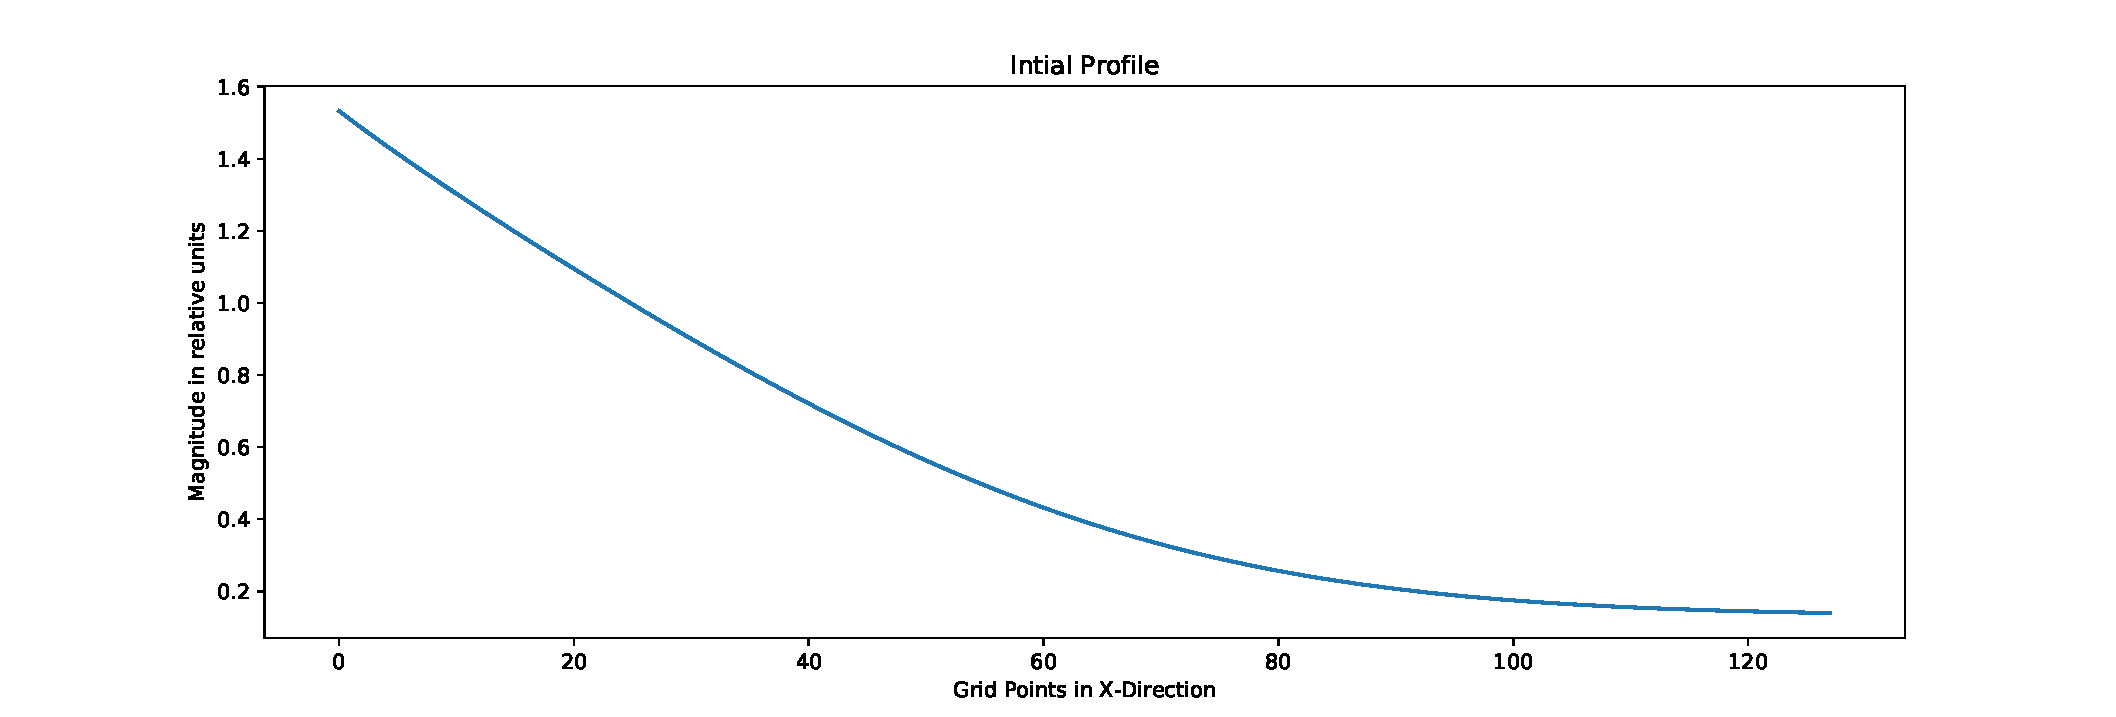
\includegraphics[width=\linewidth]{pdfs/initial_profile.pdf}
    \caption{Initial profile from initial electron and ion density is derived.}
    \label{fig:initial_profile}
\end{figure}

This data is saved as background profile to have a reference later on.
Then some fluctuations are added in the core plasma to trigger turbulence (\textit{Init::initTurbulentBath}). Afterwards the ion density is initialized:
\begin{equation}
    n_i = n_e - \frac{\tau_i \mu_i}{2} \Delta n_e
\end{equation}
This further \textit{seeds} the turbulence. The last thing to do is to set the previous time steps of the time iterators to the current value. These are considered our initial values:
\begin{equation}
    \xi^{(-i)} = \xi_{init} \colon i = 0, 1, 2
\end{equation}


\subsubsection{Restart}
On a restart the only necessary step is to initialize the time stepper since the previous steps are not stored in the data file. This creates a small error that most likely only has a small effect on the data if the simulation runs for a sufficient time afterwards but has not been evaluated properly and should be avoided. A solution would be to also save data of the previous steps.

\subsection{Gyroaveraging of Ions {\small "src/models/isothermal/gyroaveraging.cpp"}}
\label{sec:components-gryoaverage}
The work consists of applying the transformation from \autoref{eq:gyro-transformation} and then doing two Fourier transformation. Finally the result is written back. This is done in \textit{Poisson::fftwSolver2D} in file \textit{"src/algorithms/poisson/fftwsolver.cpp"}.
A second implementation is available executing the code on the GPU using the \textit{cufft}-library from the nvidia cuda toolkit. The steps are shown in \autoref{eq:gyroaveraging-steps}. The non Fourier transformation is always done on the CPU but the Fourier transformation may either be executed on the CPU or the GPU.

\begin{equation}\label{eq:gyroaveraging-steps}
    \begin{split}
    &n \overset{t}{\longrightarrow} n_t \overset{DFT}{\longrightarrow} \mathcal{F}(n_t)\\
    &\mathcal{F}(n_t) \overset{\cdot C_i}{\longrightarrow} \mathcal{F}(N_t)\\
    &\mathcal{F}(N_t) \overset{DFT^{-1}}{\longrightarrow} N_t \overset{t^{-1}}{\longrightarrow} N
    \end{split}
\end{equation}

\subsection{External Sources/Sinks {\small "src/models/isothermal/external3d.cpp"}}
\label{sec:components-external}
This step is necessary to keep the simulation stable at the edges. There is a zone on the left and on the right x-boundary that artificially forces the densities and parallel velocities to \textit{practical} values. The borders of the zone are smoothed out to prevent high gradients. At first the gyroaveraged density of the ions is forced to the background density. Afterwards $\Gamma_0^{-1}$ is applied and the other densities are forced to equal this inverse (individually for each coordinate):

\begin{equation}
    \begin{split}
        N_i &= (N_i - n_0) \cdot \alpha(x) + n_0\\
        n_s &= (n_s - \Gamma_1^{-1}N_i) \cdot \alpha(x) + \Gamma_1^{-1}N_i\\
        v_{s\parallel} &= \alpha(x) \cdot v_{s\parallel}
    \end{split}
\end{equation}
A visualization of $\alpha(x)$ is given in \autoref{fig:alphavisualization}.
\begin{figure}[!hbtp]
    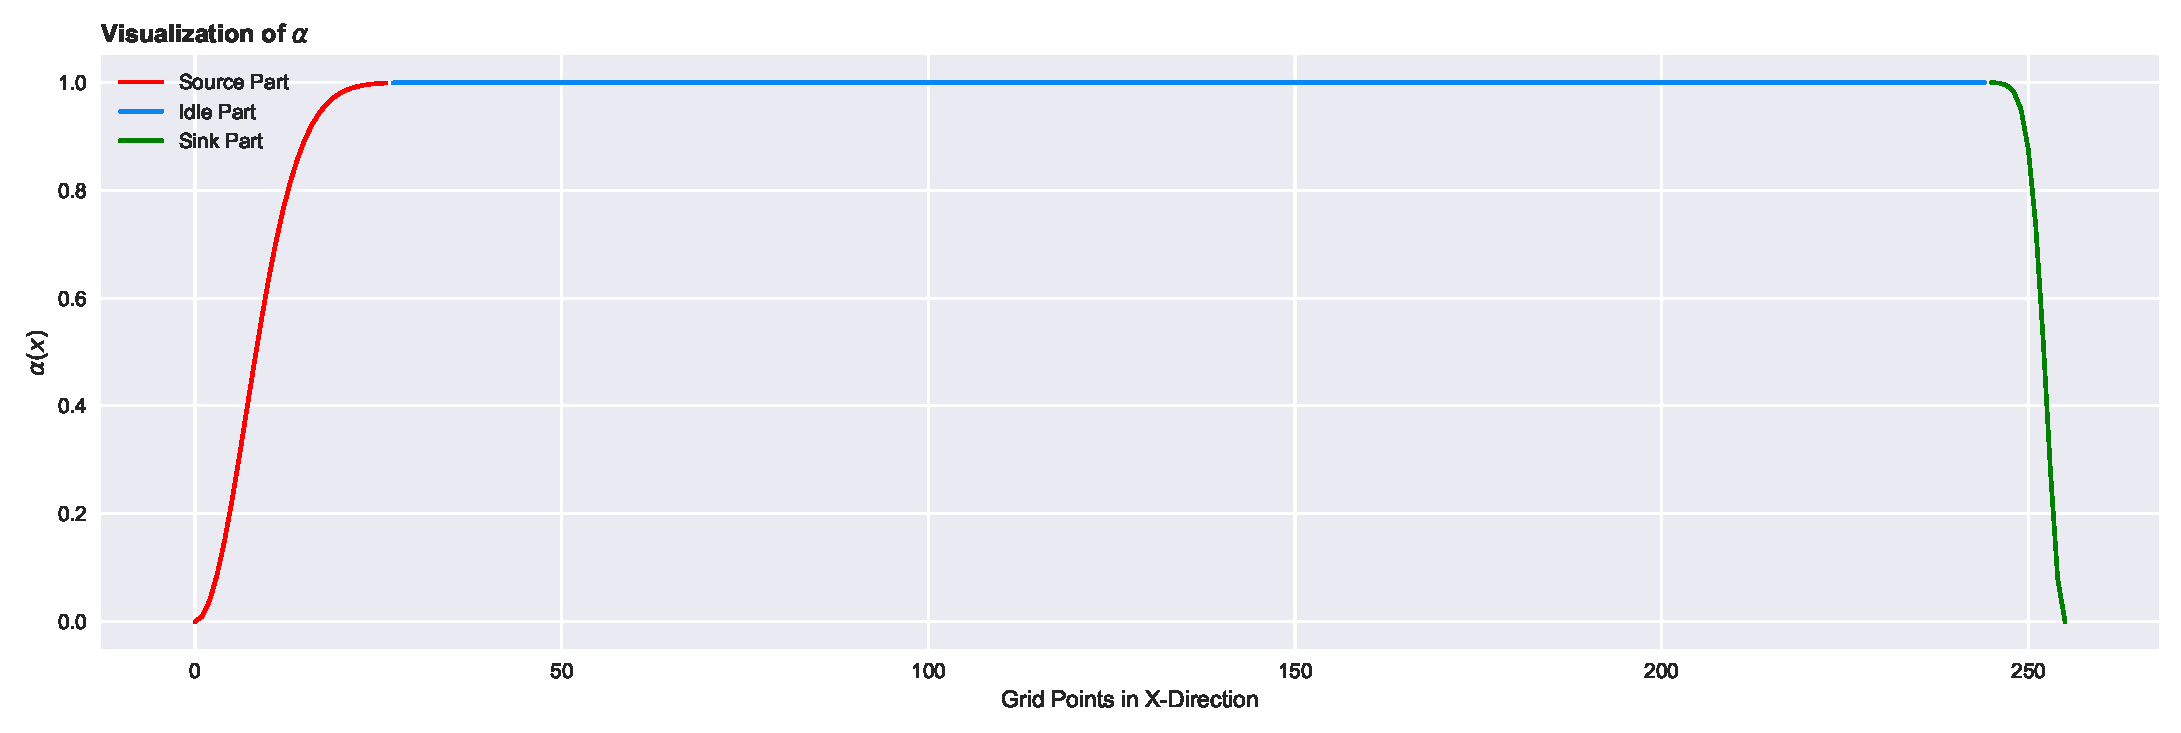
\includegraphics[width=\linewidth]{pdfs/alphavisualization.pdf}
    \caption{Visualization of $\alpha(x)$ as profile for external sources and sinks.}
    \label{fig:alphavisualization}
\end{figure}
 
 \subsection{Polarization Equation {\small "src/models/isothermal/polarization3d.cpp"}}
\label{sec:components-polarization}
The code execution is straight forward.
\begin{enumerate}
    \item Calculate right hand side ($F$) and non-linearity ($N$) of: $\nabla N \nabla \phi = F$
    \item Choose initial values of solver to be: $\phi_0 = \phi^{-1} + 0.75 \cdot (\phi^{-1} - \phi^{-2})$
    \item Execute solver (either on CPU or GPU) (\autoref{sec:sor-solver-implementation})
    \item Calculate gyro-screen potential
    \item Add a special non-linear term which is not discussed here
    \item Update potential ghost cells where necessary
\end{enumerate}


\section{SOR-Solver Implementation}
\label{sec:sor-solver-implementation}
There are two different implementations available. Both solve \autoref{eq:general-nonlinear-poisson} on a 2-dimensional grid.
\begin{equation}
    \nabla N(x,y)\nabla U(x,y) = F(x,y)\label{eq:general-nonlinear-poisson}
\end{equation}
Specific boundary conditions are employed:
\begin{equation}
    \begin{split}
        U(x, 0) &= U(x, n_y - 1) \\
        U(x, n_y) &= U(x, 1)\\
        U(0, y) &= 0\\
        U(n_x, y) &= U(n_x - 1, y)
    \end{split}
\end{equation}
Formulated in words this means that the domain is circular in y-direction, Dirichlet bound in the left-x direction and open ended in the right-x direction.
The implementation uses a Red-Black iteration scheme which allows to always use the newest data points and thus increases convergences. The algorithm first builds a linear system of equations by discretization of the non linear Poisson equation (\autoref{sec:polarization-equation}). The resulting equation
\begin{equation*}
    AU = F
\end{equation*}
is then solved using the \ac{SOR} \cite{SORPaper} method.

\subsubsection{CPU Implementation}
On the CPU the red black scheme is implemented by two sweeps over the complete matrices. The inner loop over the y dimension is vectorized by the compiler. The implementation is straight forward and easy to understand.

\subsubsection{GPU Implementation}
On the GPU a different approach has been taken. Since it is faster to load adjacent data points into shared memory (coalesced memory access) it is useful to rearrange the data and split them into two matrices. One containing all the red (even) data points and the other all black (odd) data points. The implementation follows the one presented in this conference article \cite{CUDARedBlack}.

\section{Modularization}
A moderately high level of abstraction is employed in the code base to allow modularization. In this context this means that specific parts of the code are easily interchangeable with newer/other implementations. To make this possible the components may only be loosely coupled. \autoref{fig:highLevelCodeStructure} shows the general structure of the code. Now it can easily be seen that the implementation of a new model can simply reuse \textit{Algorithms, Domain and Core} modules of the existing models. Furthermore one can for example improve the algorithms without greater knowledge about the model since the algorithms do not depend on the models. Also the implementation of newer models does not interfere with the function of the existing models.
\begin{figure}[h]
    \centering
    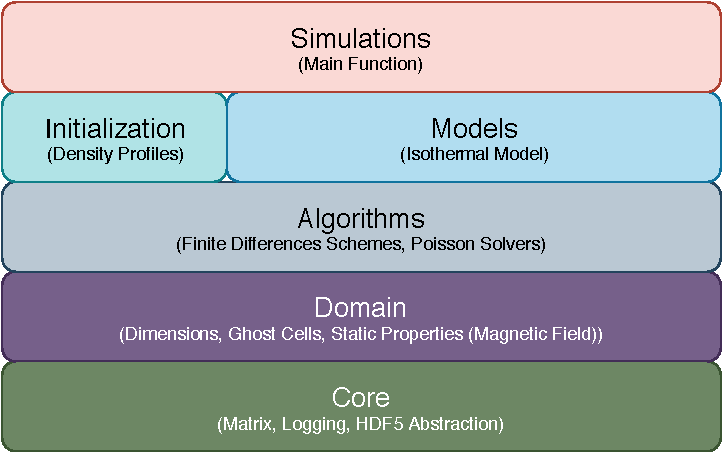
\includegraphics[]{pdfs/code_modules_high_level.pdf}
    \caption{High level structure of code. Each module may only depend on all beneath it.}
    \label{fig:highLevelCodeStructure}
\end{figure}

\section{Input}
The simulation parameters are provided via a \ac{JSON} configuration file. The default file name is \textit{"config.json"} but one may specify another file using the \textit{"-c <config-file>"} command line option. The available parameters are described in the wiki of the repository (\href{https://git.uibk.ac.at/csat8630/t3g-cmake/wikis/parameters}{Link-Wiki-Repository}). It is also possible to restart computation from a data file using \textit{"-r <data-file>"}. This restarts from the last saved iteration. One may also provide a specific data set to restart from using \textit{"-s <iteration-number>"}. For Example:
\begin{quote}
    \small
./Isothermal3d -r "\url{~/data/specialRun.hdf5}" -s 10001
\end{quote}
or even restart with new parameters:
\begin{quote}
\small
      ./Isothermal3d -c "\url{~/configs/specialRun2.json}" -r "\url{~/data/specialRun.hdf5}" -s 10001  
\end{quote}
A running simulation can not be changed though this may be implemented quite easily.

\section{Output}
\label{sec:output}
The output is collected into a single \ac{HDF5} file. The structure for the Isothermal model simulation is discribed here \textit{\href{https://git.uibk.ac.at/csat8630/t3g-cmake/wikis/Isothermal/Output}{Wiki Isothermal Output}}.

\section{Python Plotter}
The repository contains a small python application to visualize data. It uses \textit{PyQt5} and \textit{matplotlib}. It is found in the folder \textit{"plotter"} and can be started using
\begin{quote}
    python main.py
\end{quote}
in a suitable environment. The application creates 2D heatmaps of the densities, parallel velocities, potential and vorticity as well as radial profiles. Further more it can plot the energetics output.

\end{document}



\chapter{Performance Optimizations}
\subfile{performanceOptimization}
% \documentclass[master.tex]{subfiles}
 
\begin{document}


In this chapter the used optimization methods are described and evaluated. Since a deeper discussion would be out of scope only a brief overview is given. Currently almost 50\% of the simulation time is spend on the SOR-Solver for the polarization equation. As a consequence most of the work was spend on the SOR-Solver.
\section{OpenMP}
The complete calculation of the \ac{rhs} for the density and parallel velocities equations can be parallelized without negative consequences. Most gain gives us the parallelization over the z-direction. This is achieved with a simple OpenMP \textit{"for"} worksharing construct as is it is described in \autoref{sec:open-mp-method}. Parallelization in x-direction is only effective for 2D simulations or for very high resolutions. Using the construct on the y-direction is not useful since this loop is always vectorized by the compiler yielding much higher performance. Since the SOR-Solver only works in xy-direction the parallelization in z-direction is effective as well.

\section{Nvidia-CUDA}
To further optimize the SOR-solver and reduce execution time the iteration is moved to the graphics card. This creates some overhead since data has to be moved back and forth to the GPU. Also since there is usually only one GPU available the parallelization in z-direction is not possible anymore. Scaling for different systems is presented later.

\section{Evaluation}
To evaluate performance in a realistic situation it is measured using an actual simulation. A single measurement consists of 1000 iterations where the execution time is measured each 20 iterations. Also measured is how much the different steps of each iteration take.\newline
The code is evaluated on three different systems:
\begin{itemize}
    \item \textbf{\ac{K40}}: Intel Xeon E3-1225 V2; 16GB RAM; Nvidia K40
    \item \textbf{\ac{GTX}}: 2x Intel Xeon Bronze 3104; 12x 8GB RAM; 7x Nvidia GTX 1080 Ti
    \item \textbf{\ac{TV}}: 2x Intel Xeon Gold 6130; 12x 16GB RAM; 4x Nvidia Titan V
\end{itemize}
Two versions are tested against each other. The first version only runs on the CPU. The second version executes the \ac{SOR}-Solver and the Fourier transformation associated with gyroaveraging on the GPU(s). Both versions are compiled with \textit{-march=native -O3} and for the different systems the corresponding cuda compute architecture versions. Four different resolutions (z,x,y) are tested:
\begin{enumerate}
    \item 8x128x128
    \item 8x128x256
    \item 8x256x512
    \item 8x512x1024
\end{enumerate}

\subsection{Data Output}
Five sections of the code are measured individually as well as the global execution time:
\begin{itemize}
    \item Polarization Equation
    \item Gyroaveraging
    \item Right Hand Side (RHS) of Equations (\textit{calculation of $F(\Phi)^{n+1}$ in \autoref{eq:karnidakis-scheme}})
    \item Time Stepping (\textit{Calculation of \autoref{eq:karnidakis-scheme}}
    \item External Boundaries
\end{itemize}
Each data point taken is the mean value out of 20 iterations. In \autoref{fig:k40_gpu_vs_cpu} the complete data set for 8x128x128 on the \ac{K40} and \ac{K40C} systems is presented. It is clearly visible that the first point represents an outlier which is explained by the fact that the initial value for the polarization solver is far off from the solution. It is therefor excluded from further evaluations. 

\begin{figure}[!hbtp]
    \centering
    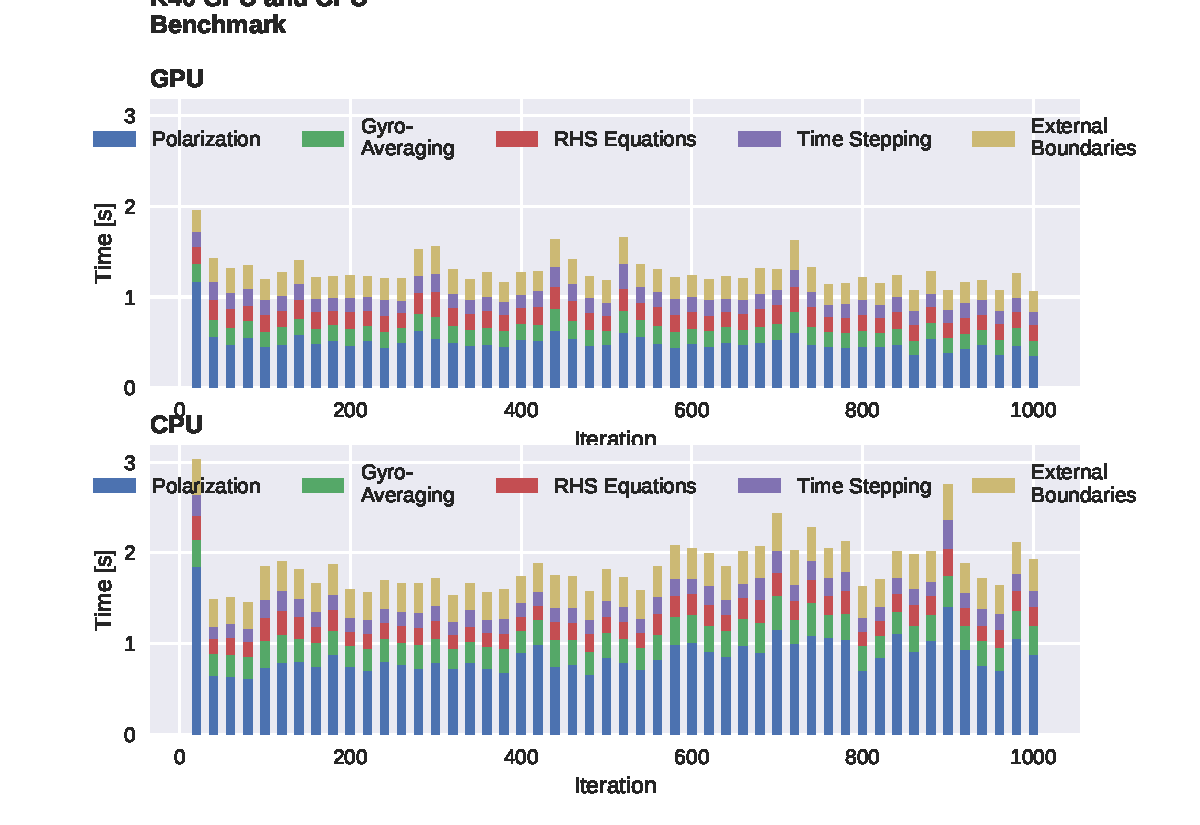
\includegraphics[width=\linewidth]{pdfs/k40CPUvsGPU_full.pdf}
    \caption{\small Example of performance run. Timings are taken every 20 iterations. Comparison for 8x128x128 on K40 workstation}
    \label{fig:k40_gpu_vs_cpu}
\end{figure}

\autoref{fig:k40_gpu_vs_cpu_mean} shows the mean duration of each step. There is no significant difference visible in "Time Stepping" and "RHS Equations". This is expected since both steps are fully executed on the CPU. One can however already see a performance improvement for the other steps. \autoref{tab:talbe_k40_k40c} presents the quantitative results. The GPU scales better with grid size even though this is a perfectly parallelizeable problem for the CPU where each core calculates one xy-layer in z-direction. Speedups >2 are observed.
The larger errors assoicated with the CPU version especially for the polarization may be explained by the scheduler of the operation system. More information on scheduling on linux systems and the negative impact can be found here \cite{Scheduling-Linux}.

\begin{figure}[!hbtp]
    \centering
    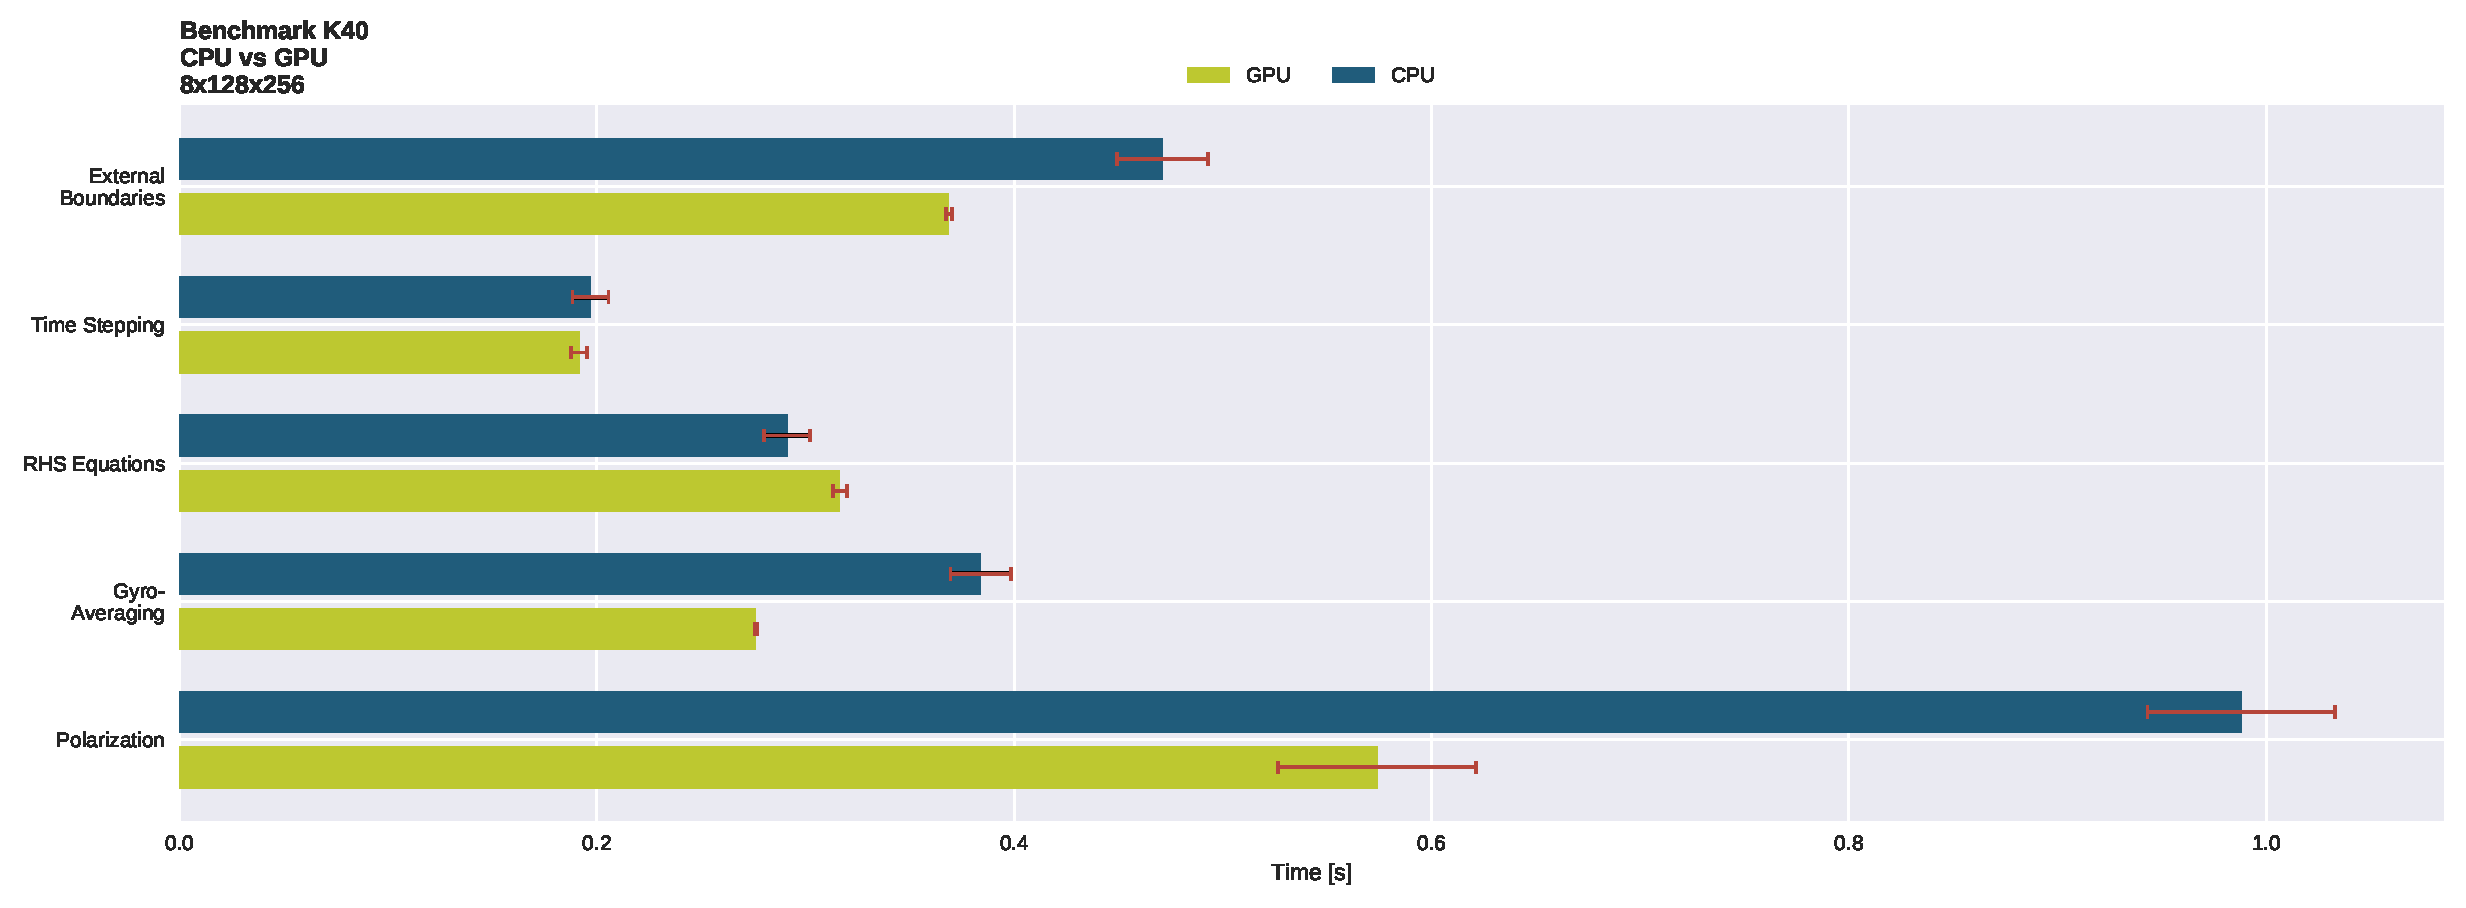
\includegraphics[width=\linewidth]{pdfs/k40CPUvsGPU_means.pdf}
    \caption{\small Mean and standard deviation of timings measurement presented in \autoref{fig:k40_gpu_vs_cpu} omitting the first data point.}
    \label{fig:k40_gpu_vs_cpu_mean}
\end{figure}

\begin{figure}[!hbtp]
    \centering
    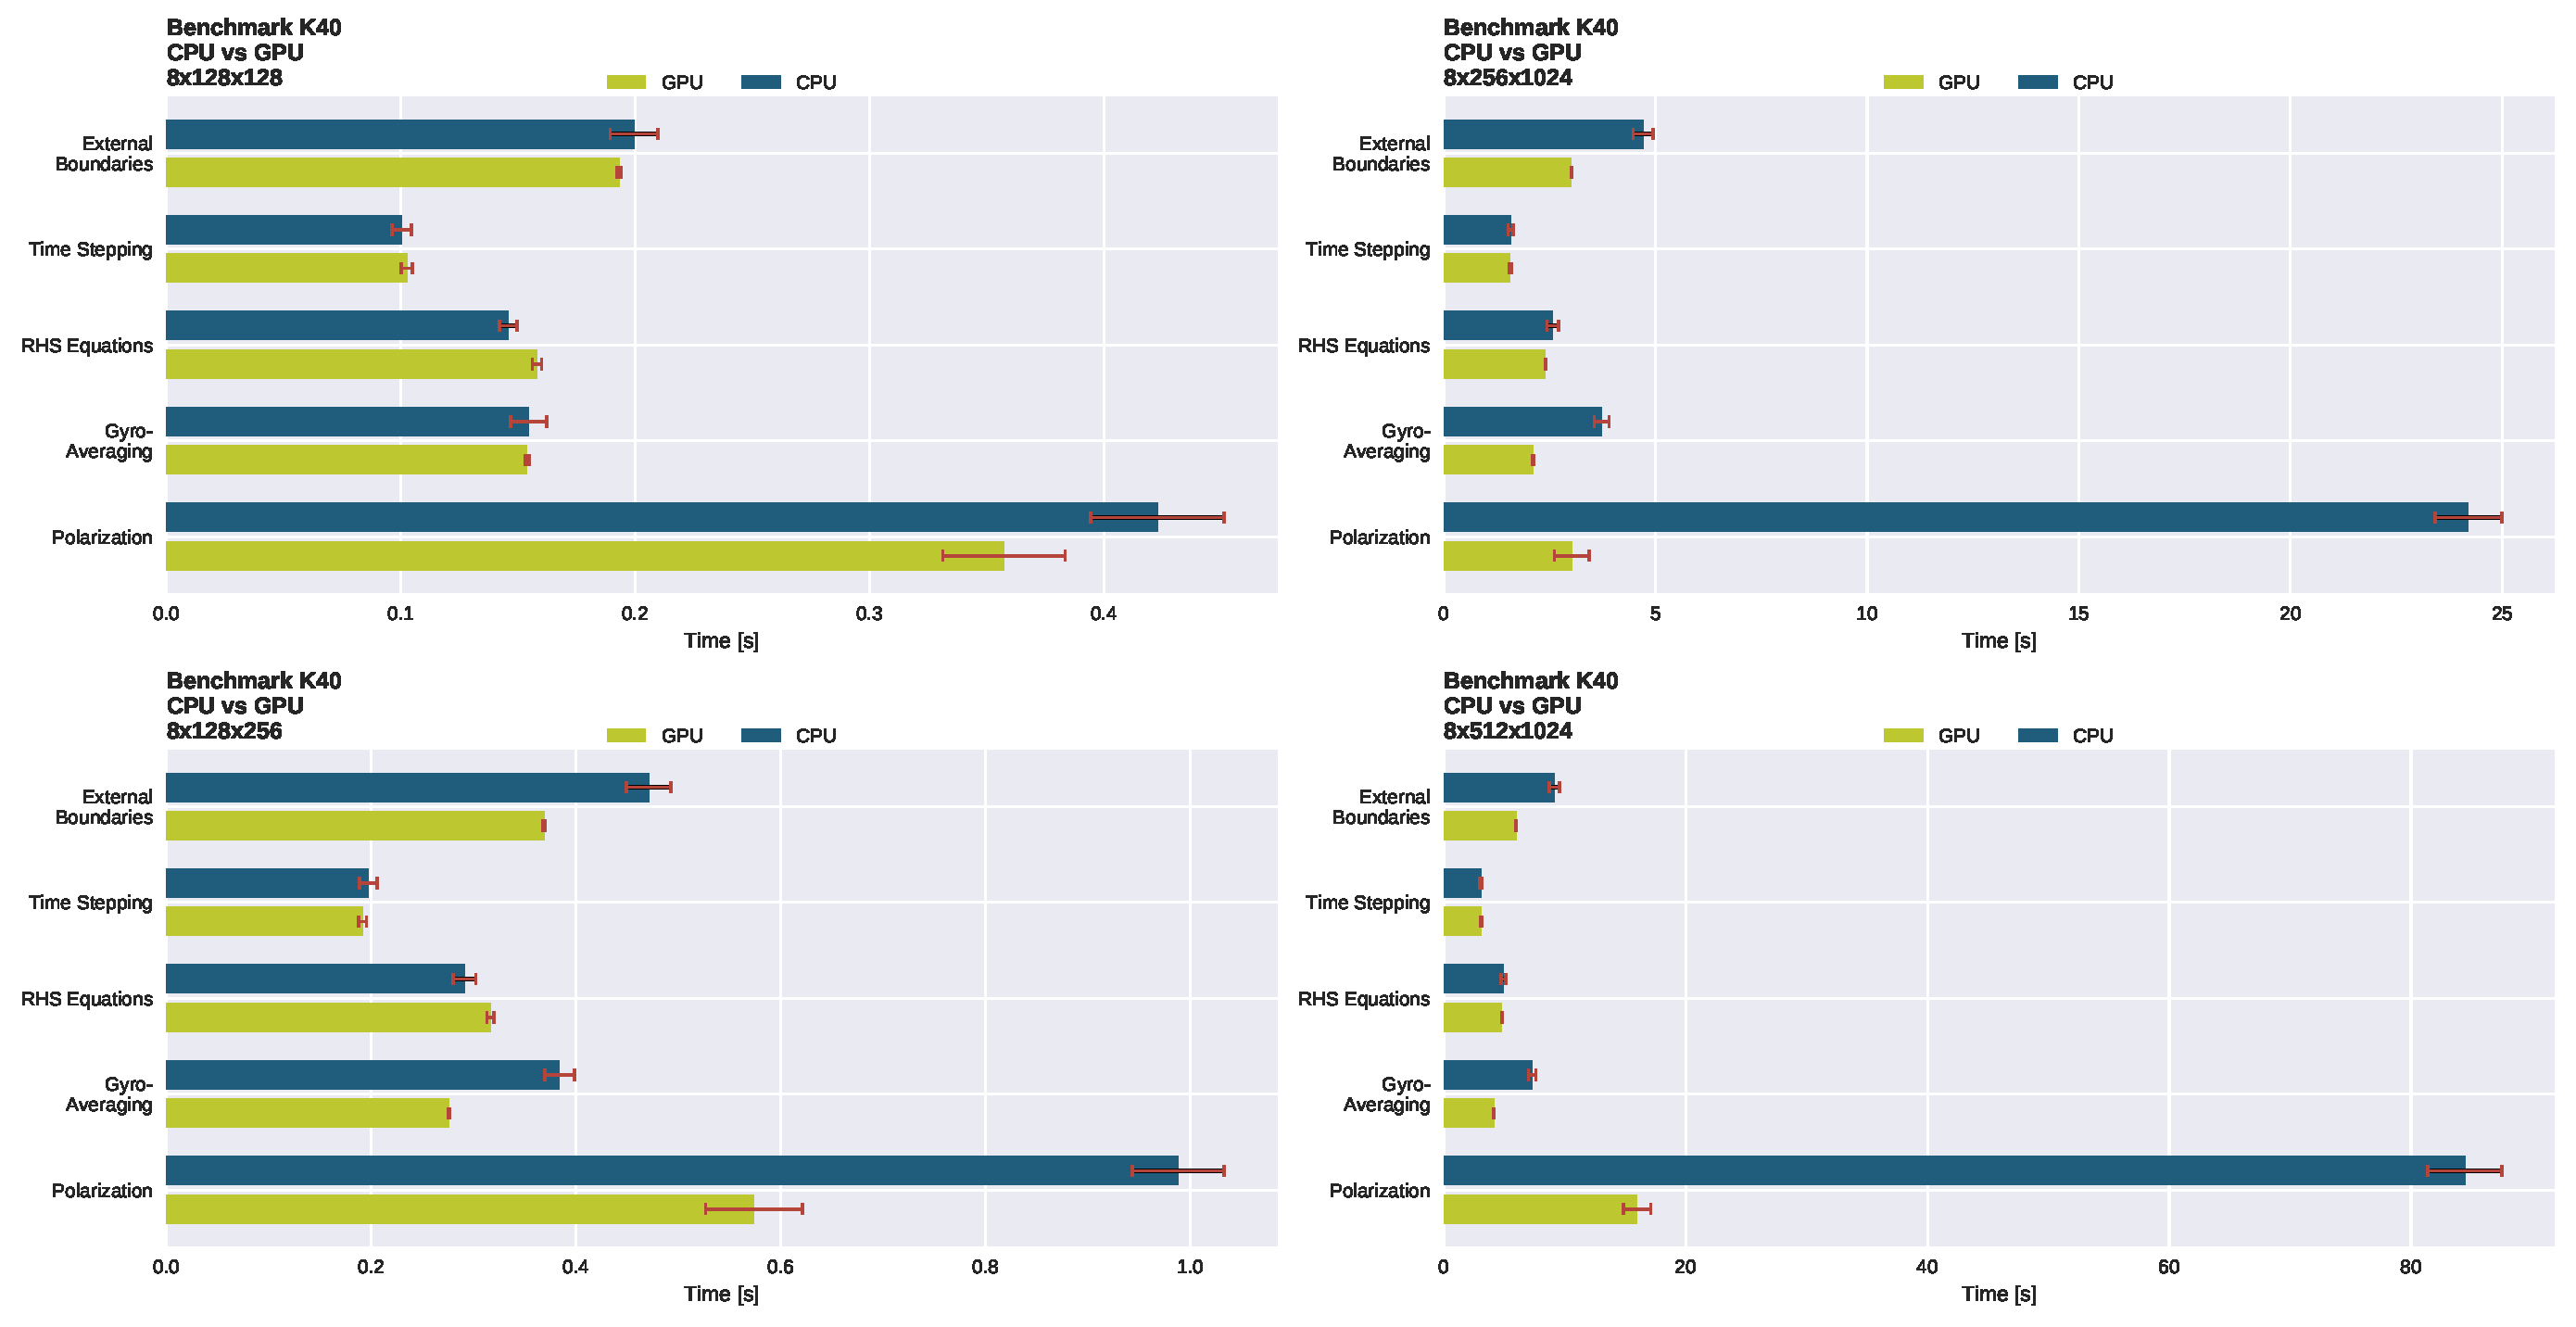
\includegraphics[width=\linewidth]{pdfs/k40CPUvsGPU_complete_means.pdf}
    \caption{\small Comparison of \ac{K40} and \ac{K40C} for all resolutions.}
    \label{fig:k40_gpu_vs_cpu_complete_means}
\end{figure}

\begin{table}[!hbtp]
    \centering
    \begin{tabular}{c|c|c|c}
        Grid Size & \ac{K40} & \ac{K40C} & GPU Speedup  \\  \hline
        8x128x128 & $1.89 \pm 0.28$s & $1.32 \pm 0.15$s & $1.43 \pm  0.27$ \\
        8x128x256 & $3.76\pm0.42$s & $2.38\pm0.19$s & $1.58\pm0.21$ \\
        8x256x512 & $17.92\pm4.13$s & $8.10\pm0.40$s & $2.21\pm0.52$ \\
        8x256x1024 & $36.27\pm8.19$s & $16.85\pm0.76$s & $2.15\pm0.50$ \\
        8x512x1024 & $70.05\pm25.02$s & $40.45\pm2.84$s & $1.73\pm0.63$
    \end{tabular}
    \caption{Execution times of 20 iterations for \ac{K40} and \ac{K40C} and speedup of GPU version against CPU version}
    \label{tab:talbe_k40_k40c}
\end{table}
\newpage
\subsection{Results for Multi GPU Systems}
Further on results for multi gpu systems are presented. For each system the execution time using only the CPU is compared to the execution time where all available GPU devices are used as well. The results for mean execution time of 20 iterations (again omitting the first 20) are plotted in \autoref{fig:all_systems_resolution_scaling}. Generally the CPU version scales worse than the GPU version. The GTX node almost reaches a speedup of three compared to the CPU version. Considering the execution time of almost ~3s per iteration, running a simulation with 200.000 iterations takes 
almost seven days using the CPU version whereas it only takes two and a half days using the GPU version. 
\begin{figure}[!hbtp]
    \centering
    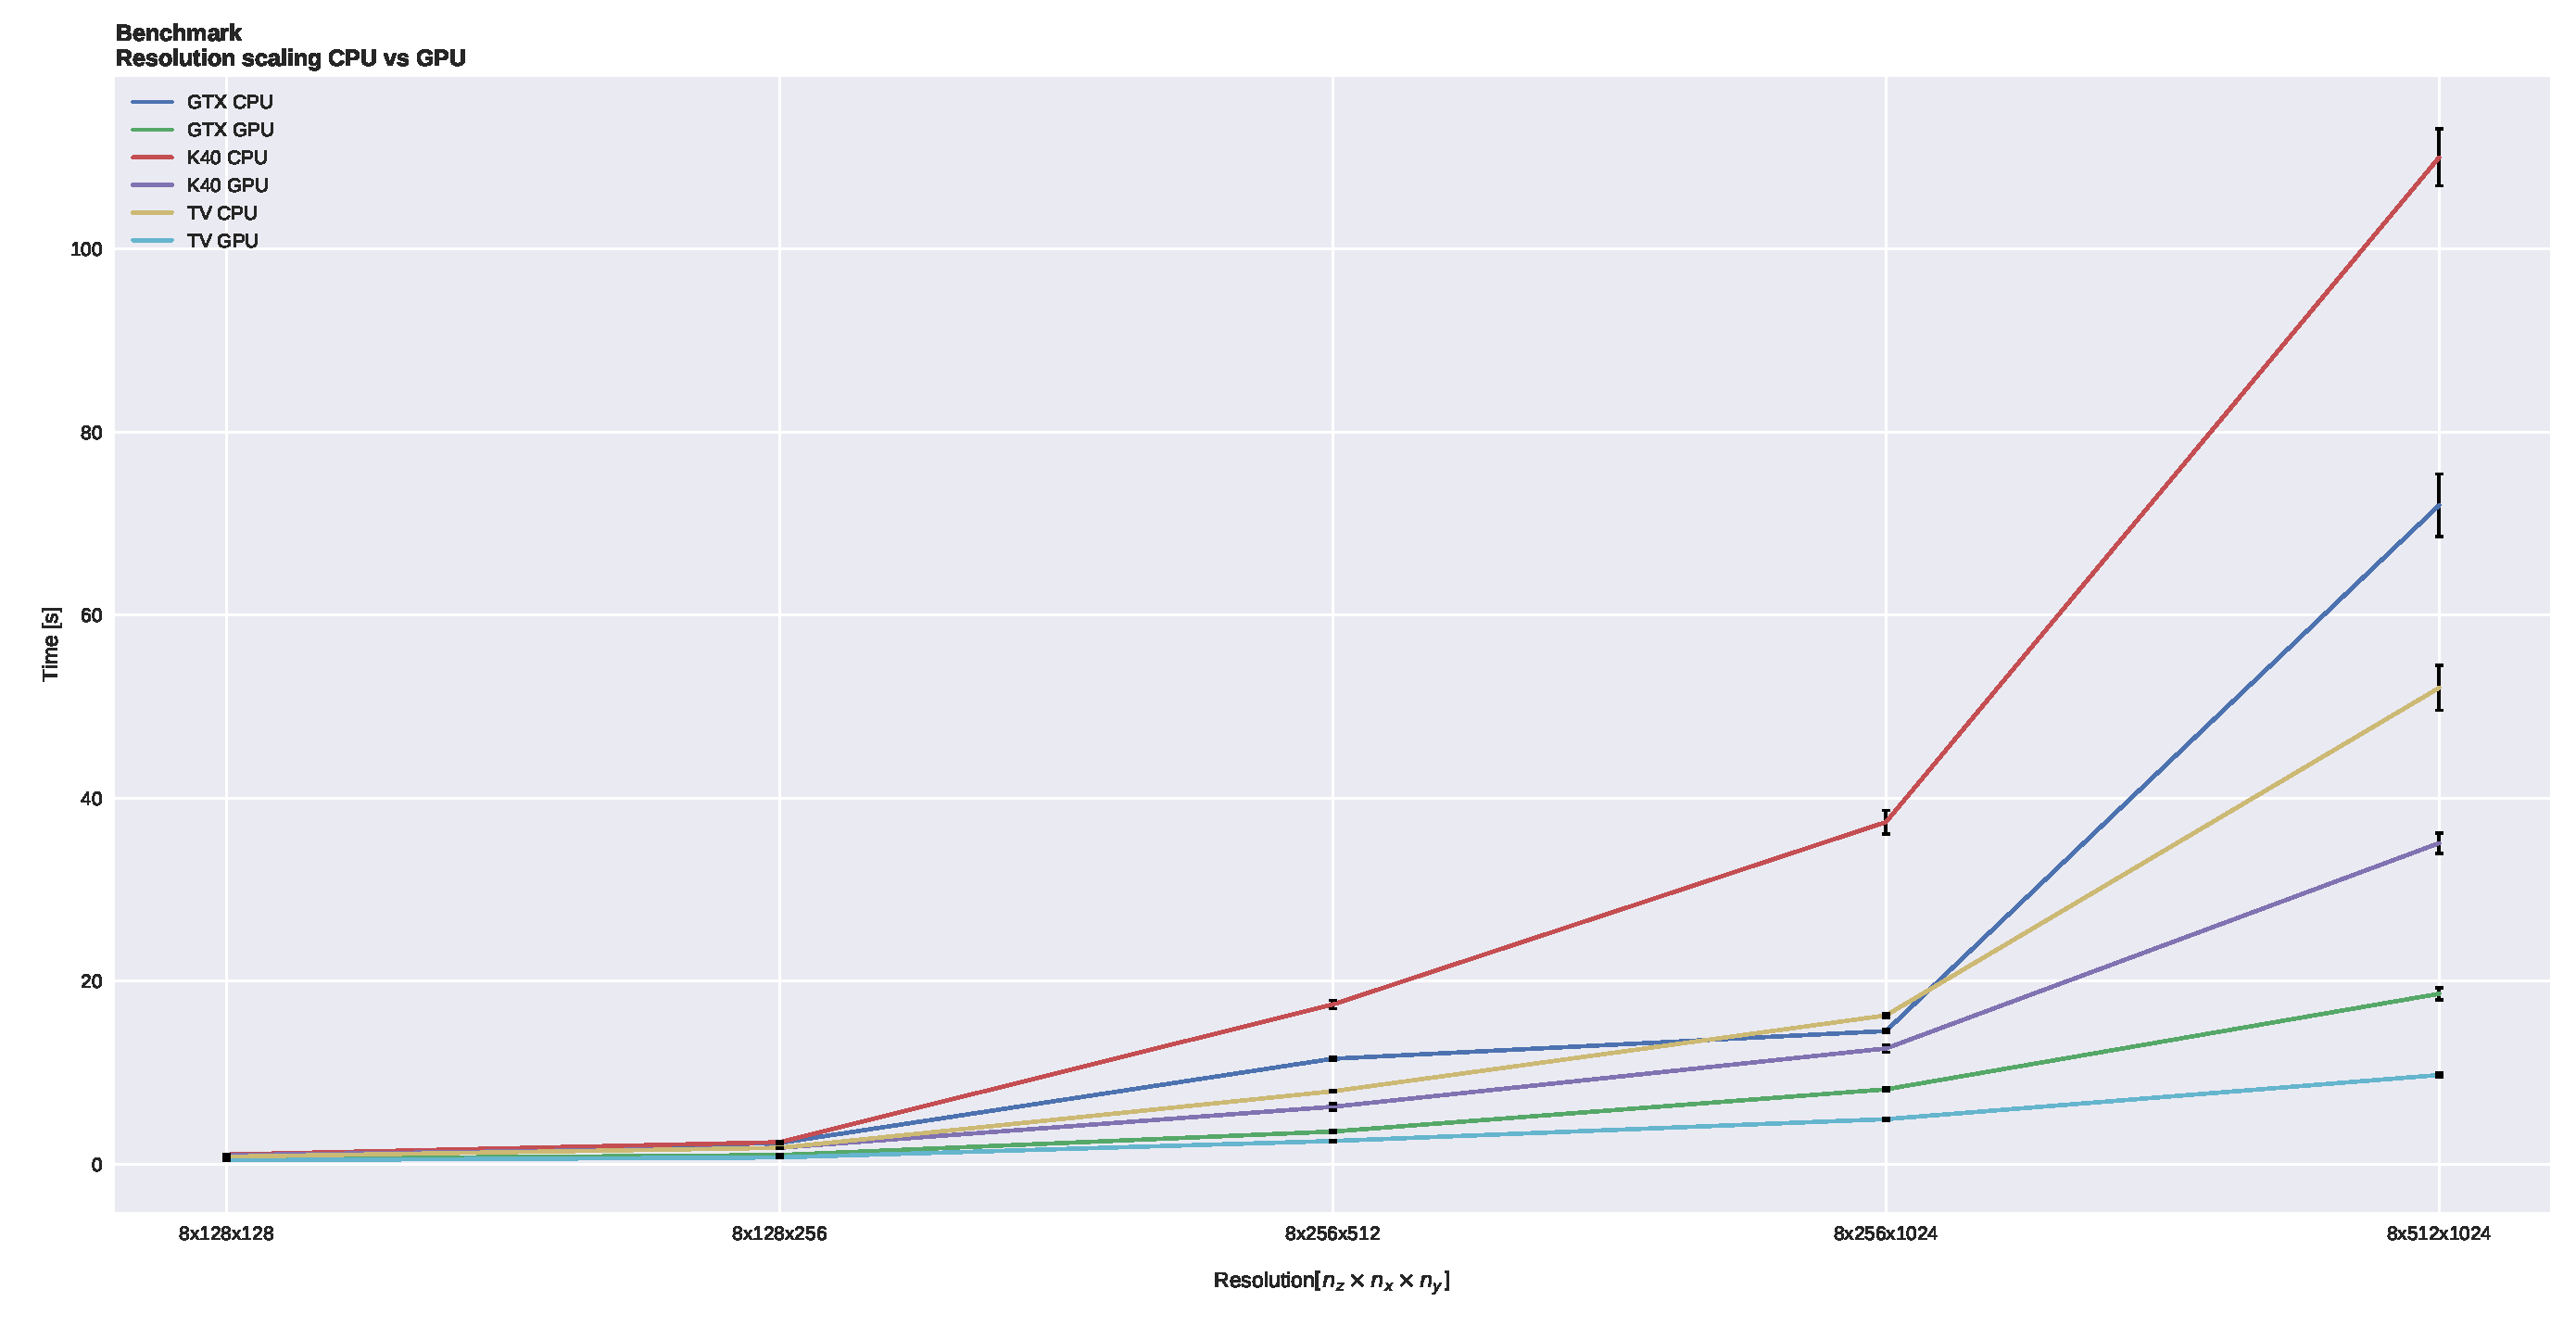
\includegraphics[width=\linewidth]{pdfs/all_systems_compared.pdf}
    \caption{\small Resolution scaling on all three systems. The GPU version genrally scales better.}
    \label{fig:all_systems_resolution_scaling}
\end{figure}

\subsection{Future Optimizations}
Using this data one can now determine where it is useful to do future optimizations. If we look at the normalized data from the \ac{GTX} system for a resolution of 8x256x1024 one can see that the most expensive part now became the time stepping (\autoref{fig:gtx_parts}).
\begin{figure}[!hbtp]
    \centering
    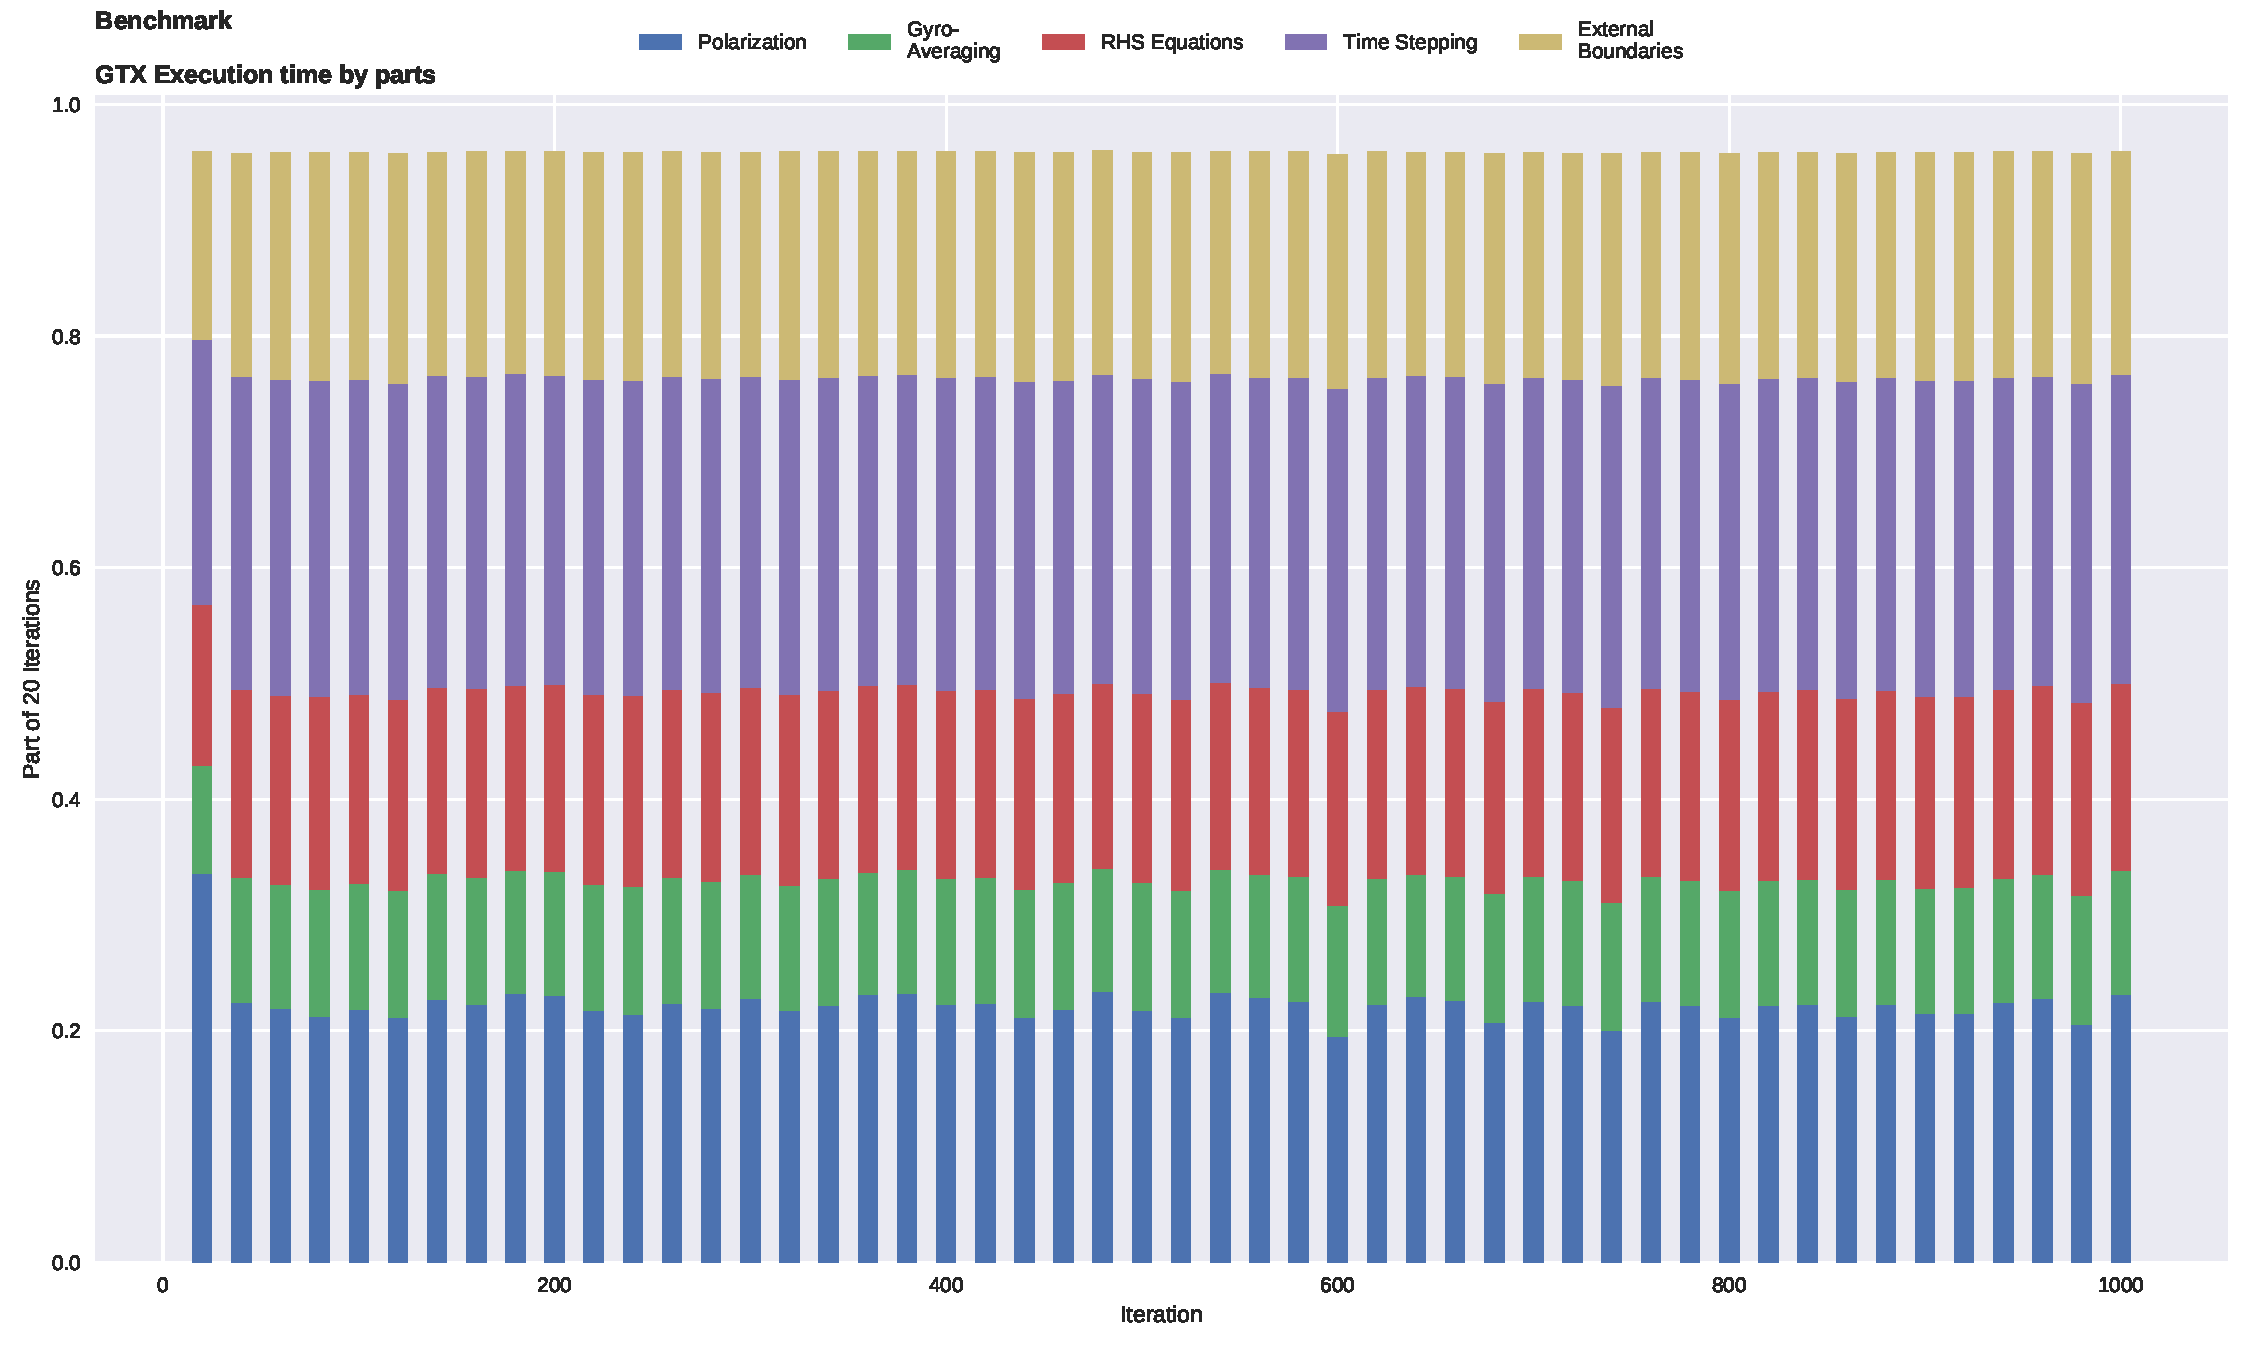
\includegraphics[width=\linewidth]{pdfs/gtx_parts.pdf}
    \caption{\small Execution times of 20 iterations normalized to the full execution time of these 20 iteartions.}
    \label{fig:gtx_parts}
\end{figure}
Moving the timestepping to the GPU as well as the \ac{RHS} evaluation would effectively fully move the simulation to GPU execution. Since less data transfers between host memory and device memory would be required this might dramatically increase performance, but data transfers between individual GPU's would be necessary to model the z-direction further increasing code complexity.

\section{Conclusion}
Speedups larger than two have been measured which at least reduces the execution time by a factor of two. The speedup is generally better the greater the grid is. This makes it possible to asses whether resolution has an impact on the simulation model. Prior to these optimization's running a simulation with grid size 8x256x1024 could take a week but is now possible in a few days allowing for faster prototyping of adjustments to the model. It should be noted though that magical speedups as they are described in \cite{CUDARedBlack} of >40 are not reached. A major positive effect on CPU performance has vectorization. Most of the simulation code is vectorized by the compiler and as such it runs very well on the CPU. Also the simulation does not have a high memory footprint since a single XY-plane takes about 2MB for a single quantity on a grid of 8x256x1024. Such a plane fits into the cache of current CPUs and naturally gives them a high memory bandwidth. Nevertheless it might be worth moving all the code to the GPU which would reduce the overhead associated with copying data from the host memory to the GPU memory. On the other hand this involves much more complex programming and in most cases exceeds the qualifications of a physicist thus making it harder to collaborate or evolve the model and simulation.



\end{document}

\subfile{polarization_equation}




\chapter{Conclusion}




\chapter{Literatur Recherche}


\newpage
\chapter{Zusammenfassung und Ausblick}

\newpage

%
% agsm in der uibk vorlage
%
% ^.

% \bibliographystyle{agsm} %apalike
\bibliographystyle{unsrt} %apalike
\bibliography{literatur}
\chapter{Acronyms}
\subfile{acronyms}
% \documentclass[master.tex]{subfiles}
 
\begin{document}

\begin{acronym}
\acro{FLR}{finite Lamor radius}
\acro{SOR}{sucessive-over-relaxiation}
\acro{JSON}{JavaScript Object Notation}
\acro{HDF5}{Hierarchical Data Format Version 5}
\acro{rhs}{right hand side}
\acro{K40C}{K40-Workstation CPU Only}
\acro{K40}{K40-Workstation}
\acro{GTX}{GTX-Cluster Node}
\acro{TV}{TV-Cluster Node}
\end{acronym}
\end{document}



\end{document}
